%% The following is a directive for TeXShop to indicate the main file
%%!TEX root = diss.tex

\chapter{A Mapping of 3D Reconstruction Techniques}
\label{ch:3DRecon_Mapping}
Most of the vision work focuses on developing algorithmic novelties, and very few investigates the rigorous conditions under which these algorithms work. Thus this knowledge is only known empirically, without a rigorous definition of the problem or application domain or the conditions. This section builds upon the 3D description proposed in Chapter~\ref{ch:3DRecon_Desc}, and attempts to find out the optimal algorithms under a pre-defined condition.

To achieve this goal, we need a dataset to evaluate the performance of each algorithm under varied conditions, which is not the goal of most of the online datasets. To the best of our knowledge, current existing 3D benchmarks focus on one specific class of algorithms, for example, the Middlebury dataset is targeted at MVS algorithms, and the `DiLiGenT' dataset is for Photometric Stereo algorithms. This makes them only suitable to the evaluation of algorithms within the same category. There is no dataset that evaluates 3D reconstruction across differ categories, let alone one that covers a range of properties and their combinations. The reasons for the lack of such dataset is: 1). it's already tedious to create a real-world dataset for a specific category of algorithms, it would be even more challenging to create a dataset for a larger range of algorithms with the ground truth; 2). it's practically impossible to make one property, \eg, noise level, lighting configuration, material, etc, varied while fixing the others in order to conduct a thorough evaluation.

We propose a synthetic but realistic (physically-based) dataset for evaluation of 3D reconstruction algorithms. The dataset includes a collection of images of a scene under different material or lighting conditions. The camera/projector intrinsic and extrinsic parameters are computed directly from the configurations of the synthetic setup, and the ground truth, including the 3D model point cloud and normal map, are generated directly from Blender.

\section{Synthetic setup}
We use the physical-based renderer Cycles in Blender to generate the synthetic dataset. For each technique, the configuration of the camera remains fixed. The image resolution is 1280$\times$720, with a focal length of $35mm$ or $1400px$.

For MVS, there are five rings of cameras, of which the elevation angle is $15^\circ$, $30^\circ$, $45^\circ$, $60^\circ$, $90^\circ$. The between-angle of two neighbouring cameras is $30^\circ$, $30^\circ$, $45^\circ$, $45^\circ$, and $360^\circ$. Thus there are in total $12+12+8+8+1=41$ cameras.

For photometric stereo, according to \cite{Berkiten:2016:ARB}, increasing the number of images is only important up to a point, the experimental results showed that most algorithms reaches to optimum when 15 images are used. To make a balance between algorithm performance and rendering time, we use 25 light sources, which are distributed on four different rings with elevation angle of $90^\circ$, $85^\circ$, $60^\circ$, and $45^\circ$. The azimuth angle between two neighbouring light sources is $45^\circ$.

For the structured light, the baseline angle between the camera and the projector is $10^\circ$, and only one camera is used, thus only a portion of the object is invisible. The resolution of the projector is $1024\times768$, thus 10 Gray code patterns are needed. To counter the effect of inter-reflection, each pattern and its inverse are projected, which makes it less sensitive to scattered light.

\section{Structure of Datasets}
Due to the number of properties and number of levels for each property, it would be unrealistic to render all the combinations of properties. For if we have $N$ properties and each is discretized into $L$ levels, the number of different combinations is $L^N$, and for each combination, there are in total $41+25+42=108$ images to render. Therefore, we take another approach: 1). first we investigate the \textit{dependency} between any two properties, if these two properties are independent, there is no need to render all their combinations whereas it's necessary to do so if they are dependent; 2). render all the dependent properties and their combinations.

\section{Selected methods}
We have selected one representative algorithm from each class of algorithms: the PMVS proposed in~\cite{furukawa2010accurate}, the example-based photometric stereo proposed in~\cite{hertzmann2005example}, and the Gray-encoded structured light technique. The current implementation of SL projects both column and row patterns, and depth values are computed using these two kinds of patterns individually. A depth consistency checking step is performed to reject erreneous triangulations.

\section{Evaluation metrics}
We use the metric proposed in \cite{seitz2006comparison} to evaluate MVS and SL algorithms. More specifically, we compute the accuracy and completeness of the reconstruction. For accuracy, the distance between the points in the reconstruction $R$ and the nearest points on ground truth $G$ is computed, and the distance $d$ such that $X\%$ of the points on $R$ are within distance $d$ of $G$ is considered as accuracy. Thus the lower the accuracy value, the better the reconstruction result. For completeness, we compute the distance from $G$ to $R$. Intuitively, points on $G$ is not ``covered'' if no suitable nearest points on $R$ found. A more practical approach computes the fraction of points of $G$ that are within an allowable distance $d$ of $R$.
Note that as the reconstruction gets better, the ``accuracy value'' goes down, but the ``accuracy'' is often claimed as improved, which is contradictory at first glance. To make it more consistent to the natural context, we say the accuracy goes up when the reconstruction gets better.

For photometric stereo, we employ another evaluation criteria, which is based on the statistics of angular error. For each pixel, the angular error is calculated as $arccos$($n_g^T n$) in degrees, where $n_g$ and $n$ are the ground truth and estimated normals respectively. In addition to the mean angular error, we also calculate the minimum, maximum, median, the first quartile, and the third quartile of angular errors for each estimated normal map.

\section{Dependency Check}
Part of the difficulty in establishing a comprehensive set of experiments for such an evaluation is the large variability of shapes and material properties. We conduct a dependency check that evaluates the performance of the algorithm by changing two properties at a time while fixing the others. The goal is to identify the dependent properties so that the dimension of the problem domain could become more manageable.

\subsection{PMVS}
We evaluate the performance of PMVS in terms of accuracy and completeness under varied combinations of properties, the settings of the properties and all their combinations are listed in Table~\ref{tab:mvs_depend_check_params}.
\begin{table}[!htbp]
  \centering
  \begin{tabular}{l*{4}{c}}
  \hline
  \textbf{Property} & Texture & Albedo & Specular & Roughness\\
  \hline
  \textbf{(a)} & [0.2, 0.8] & [0.2, 0.8] & 0.0 & 0.0\\
  \textbf{(b)} & [0.2, 0.8] & 0.8 & [0.2, 0.8] & 0.0\\
  \textbf{(c)} & [0.2, 0.8] & 0.8 & 0.0 & [0.2, 0.8]\\
  \textbf{(d)} & 0.8 & [0.2, 0.8] & [0.2, 0.8] & 0.0\\
  \textbf{(e)} & 0.8 & [0.2, 0.8] & 0.0 & [0.2, 0.8]\\
  \textbf{(f)} & 0.8 & 0.8 & [0.2, 0.8] & [0.2, 0.8]\\
  \hline
  \end{tabular}
  \caption{Property settings of the pairwise conditions used for the dependency check of the MVS algorithms.}
  \label{tab:mvs_depend_check_params}
\end{table}

\begin{figure}[!htbp]
\begin{tabular}{cc}
\includegraphics[width=0.5\textwidth]{mapping/depend_check/mvs_tex_alb}&
\includegraphics[width=0.5\textwidth]{mapping/depend_check/mvs_tex_spec}\\
(a) & (b)\\
\includegraphics[width=0.5\textwidth]{mapping/depend_check/mvs_tex_rough}&
\includegraphics[width=0.5\textwidth]{mapping/depend_check/mvs_alb_spec}\\
(c) & (d)\\
\includegraphics[width=0.5\textwidth]{mapping/depend_check/mvs_alb_rough}&
\includegraphics[width=0.5\textwidth]{mapping/depend_check/mvs_spec_rough}\\
(e) & (f)\\
\end{tabular}
\caption{Performance of PMVS under six pairwise conditions. For instance, (a) shows the performance under changing \textit{texture} and \textit{albedo} values. The property values are assigned based on (a) of Table~\ref{tab:mvs_depend_check_params}.}
\label{fig:mvs_depend_check}
\end{figure}

\subsection{Property and Reconstruction}
We investigate how each property affects the reconstruction in terms of accuracy and completeness.

\textbf{Texture} - \textit{(a), (b), (c)}. As the texture level increases, the accuracy and completeness both increase. Thus texture has a positive correlation with the accuracy and completeness of the reconstruction.

\textbf{Specular} - \textit{(b), (d), (f)}. As the specular level goes up, the accuracy and completeness of the reconstruction gets worse. Thus specular has an negative correlation with the accuracy and completeness of the reconstruction.\begin{figure}[!htbp]
\begin{tabular}{ccc}
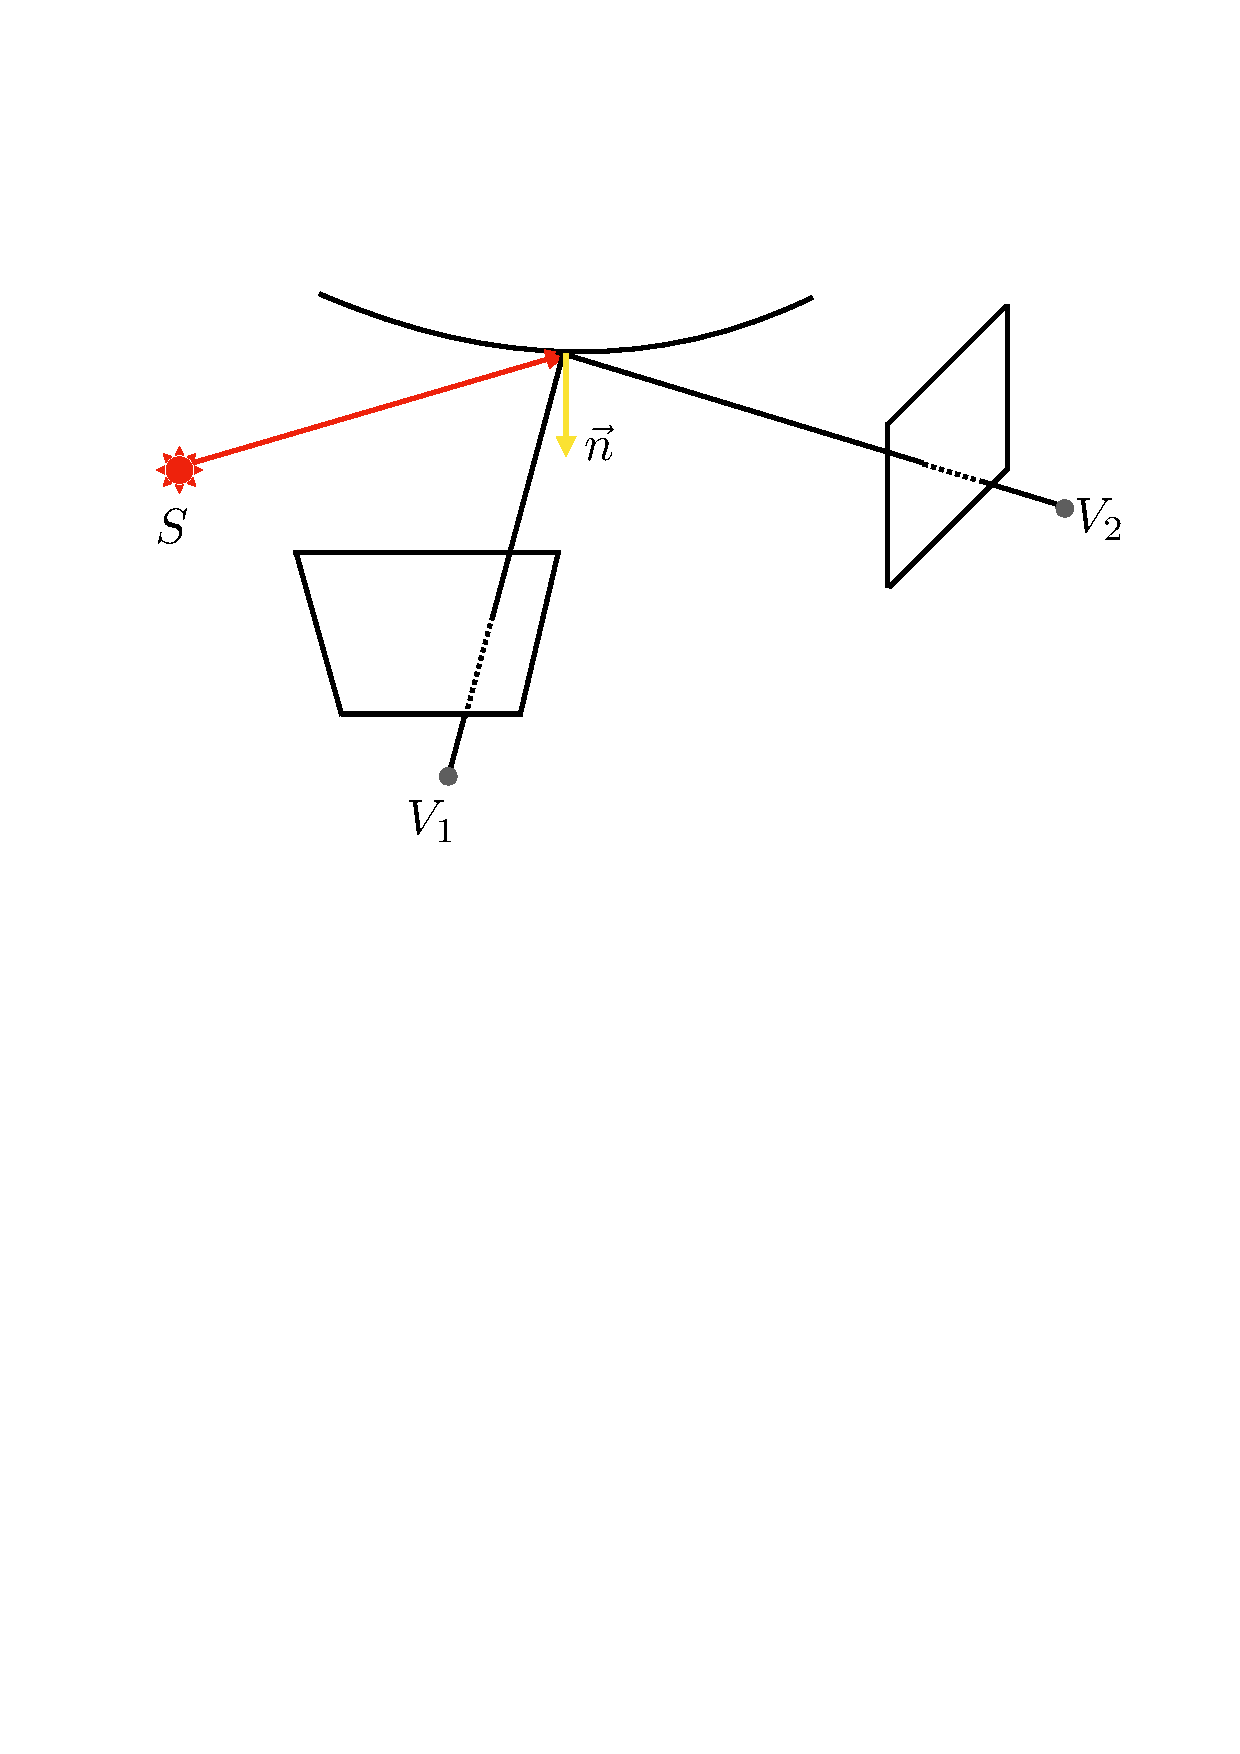
\includegraphics[width=0.33\textwidth]{mapping/mvs_spec}&
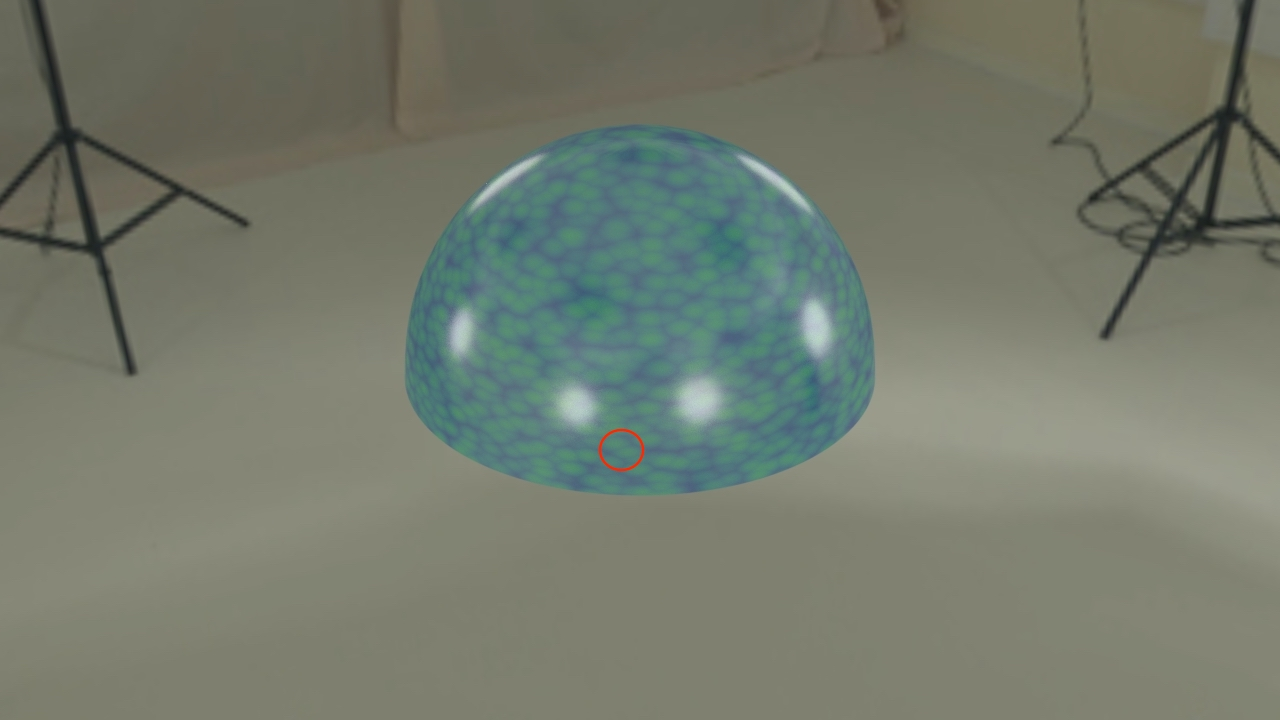
\includegraphics[width=0.33\textwidth]{mapping/mvs_spec_01}&
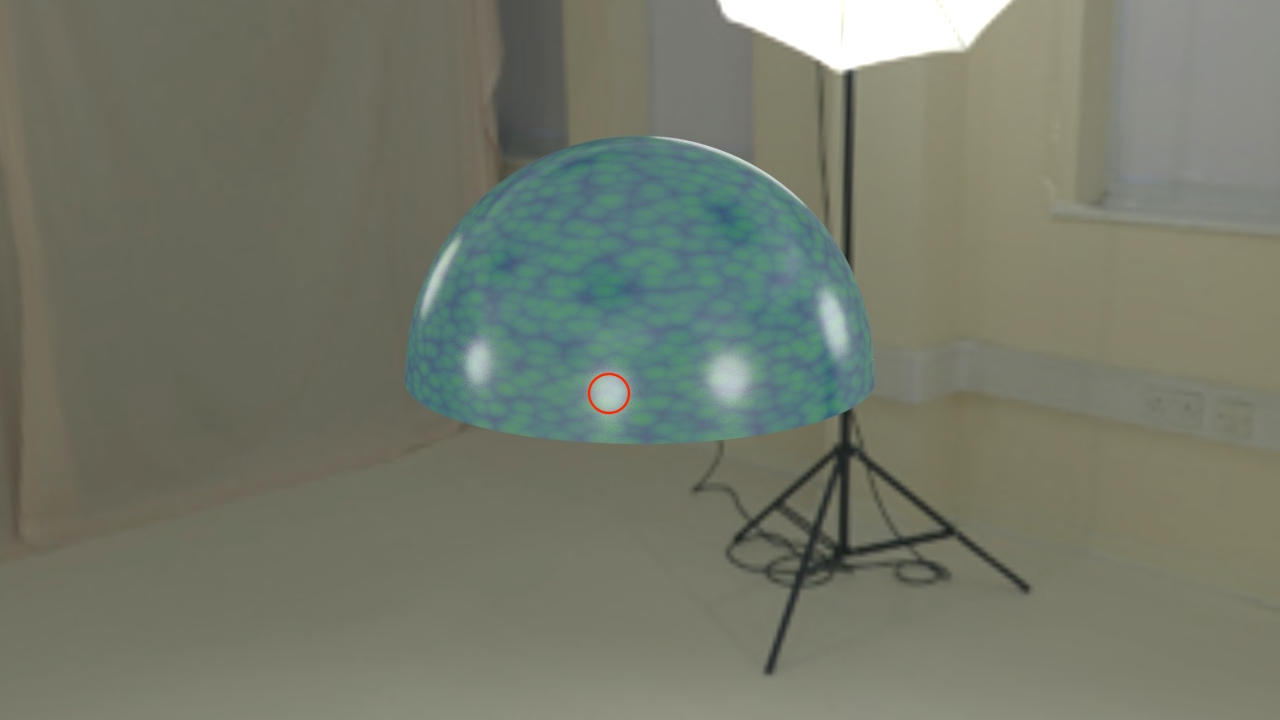
\includegraphics[width=0.33\textwidth]{mapping/mvs_spec_00}\\
(a) Image formation & (b) $V_1$ & (c) $V_2$\\
\end{tabular}
\caption{(a) shows the reflection of light off a specular surface. $V_1$ received the diffuse component while $V_2$ receives the specular component. (b), (c) shows the images observed from these two views. The specular area (red circle) observed in $V_2$ is visible in $V_1$.}
\label{fig:mvs_spec}
\end{figure}

\textbf{Texture and Specular}

\textbf{Albedo and Specular}

\textbf{Albedo} - \textit{(a), (d), (e)}. we can tell that albedo doesn't have an effect when texture or roughness changes. But when the specular level changes, albedo has an effect on both accuracy and completeness of the reconstruction.

\textbf{Roughness} - \textit{(c), (e), (f)}. We can see that roughness doesn't have a significant impact on the accuracy and completeness of reconstruction.

\subsubsection{Pairwise properties}
Now let's investigate the influence of pairwise properties. We observed that (b), and (d) has significant changes in terms of accuracy and completeness when one property changes while the other is fixed.

\textbf{(b) Texture and Specular} 
For a fixed texture, as the specularity goes up, the accuracy and the completeness goes up, which is consistent to previous observations. Besides, for a lower value texture, the effect of specular is more substantial than that for a higher value texture. However, we observe that, the specular has a bigger impact on lower textured surface, this can be explain as: the specular lobe is observed only by cameras positioned and oriented towards the specular lobe, thus only a highlight is visible. Thus cameras positioned otherwise would observed the true surface. The reconstruction exploit the texture information provided by those latter cameras, and thus is able to reconstruct the specular surface. If the surface texture level decreases, as shown before, the reconstruction deteriorates.

\textbf{(d) Albedo and Specular} 
For a fixed albedo, as the specular goes up, the accuracy and completeness both goes down, which is consistent to previous observations. However, the effect of specular is more substantial for a lower value albedo than that for a higher value albedo.
\begin{figure}[!htbp]
\centering
\begin{tabular}{ccc}
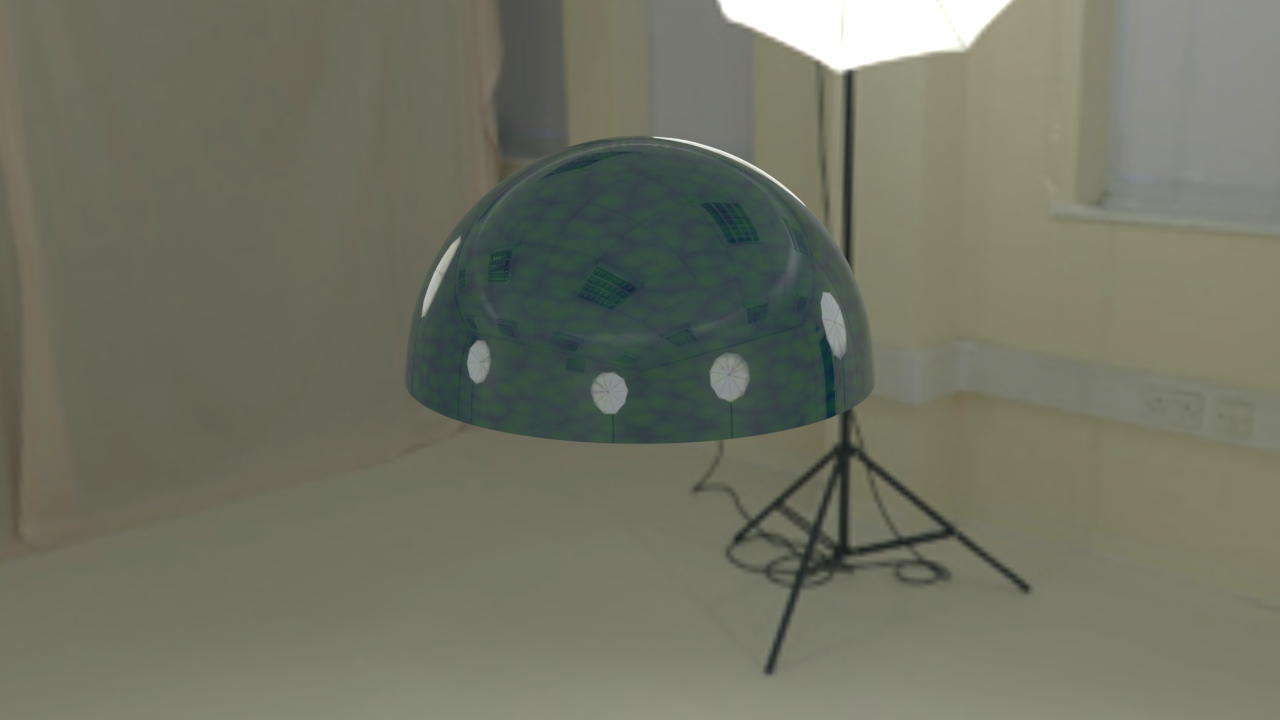
\includegraphics[width=0.33\textwidth]{mapping/mvs_alb_spec/alb_spec_0202}&
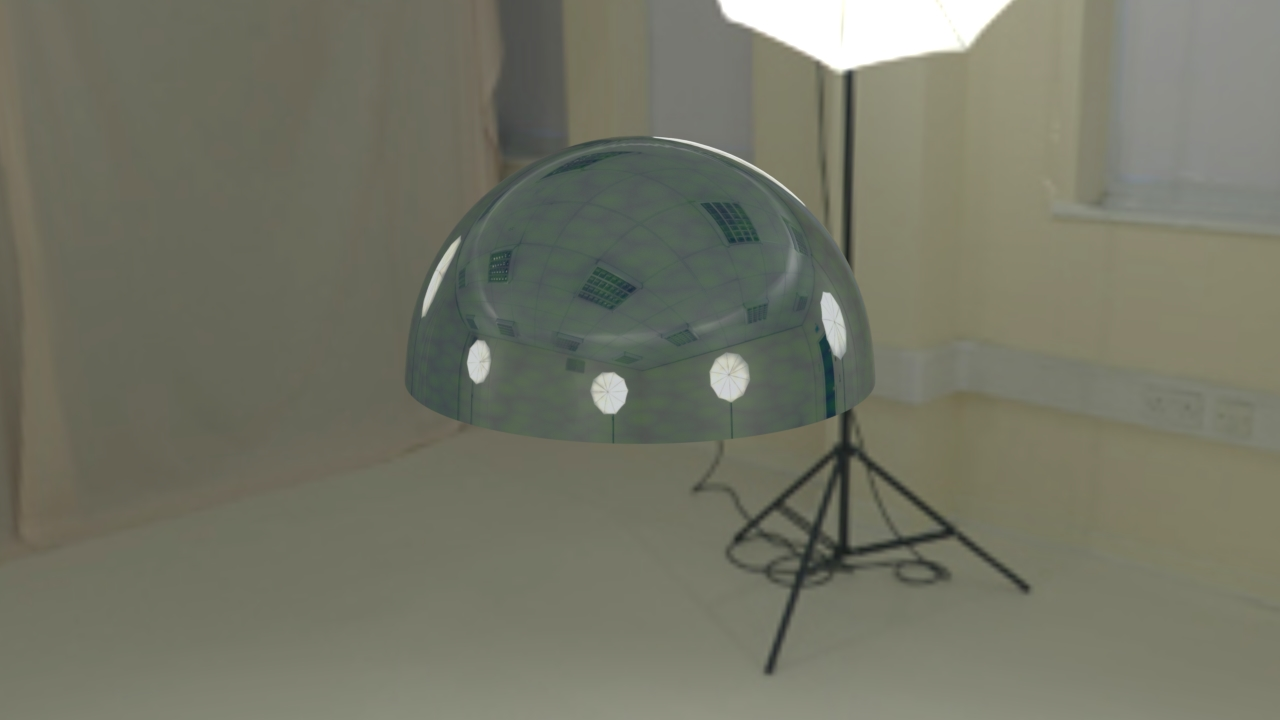
\includegraphics[width=0.33\textwidth]{mapping/mvs_alb_spec/alb_spec_0205}&
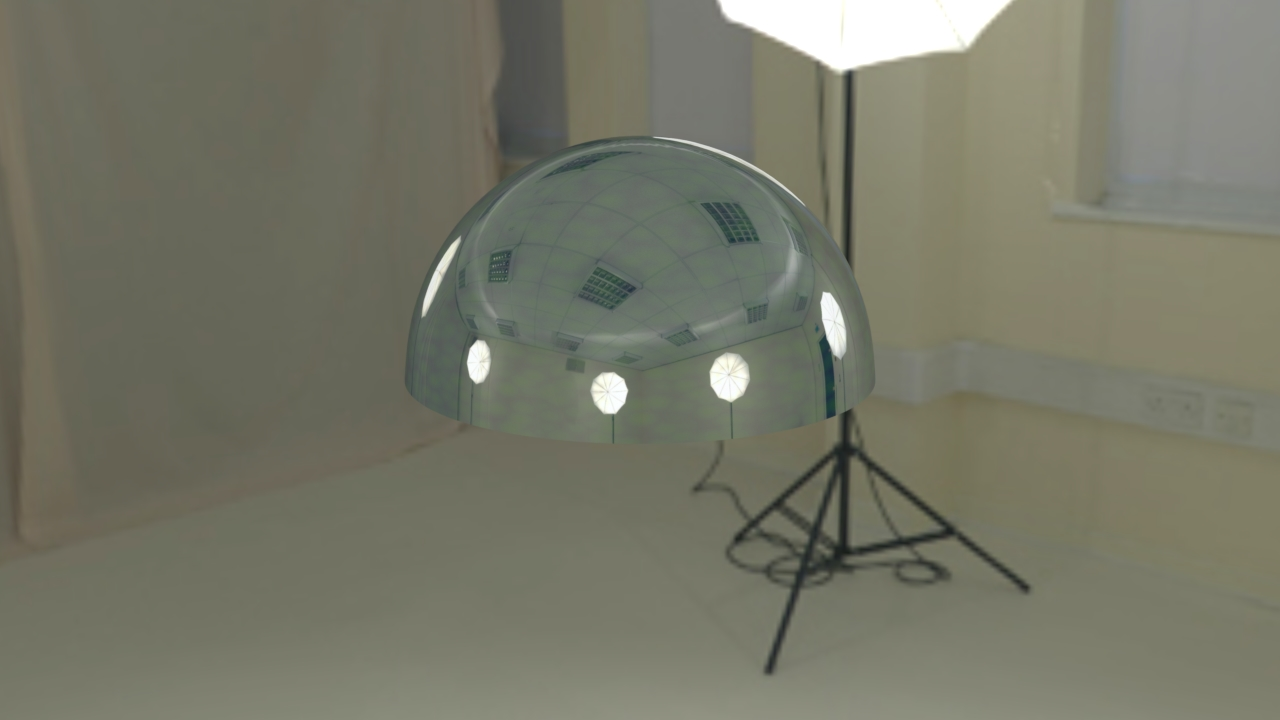
\includegraphics[width=0.33\textwidth]{mapping/mvs_alb_spec/alb_spec_0208}\\
(a) spec: 0.2 & (b) spec: 0.5 & (c) spec: 0.8\\
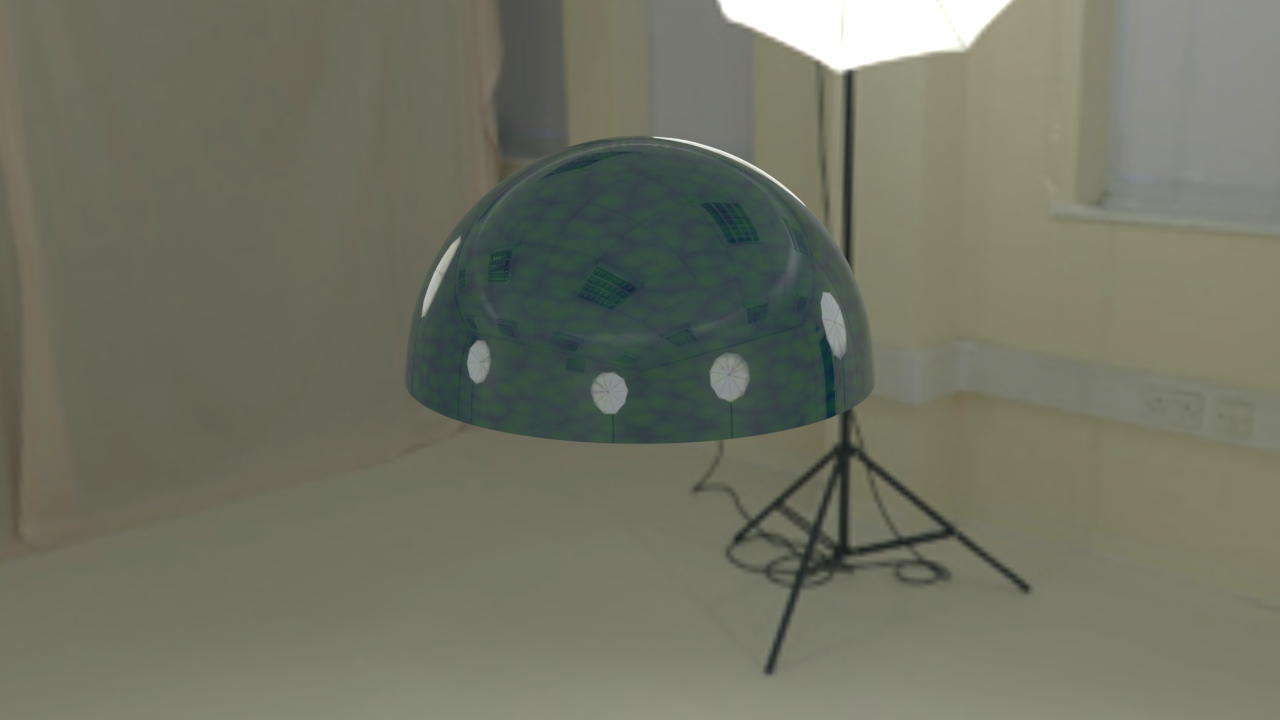
\includegraphics[width=0.33\textwidth]{mapping/mvs_alb_spec/alb_spec_0202}&
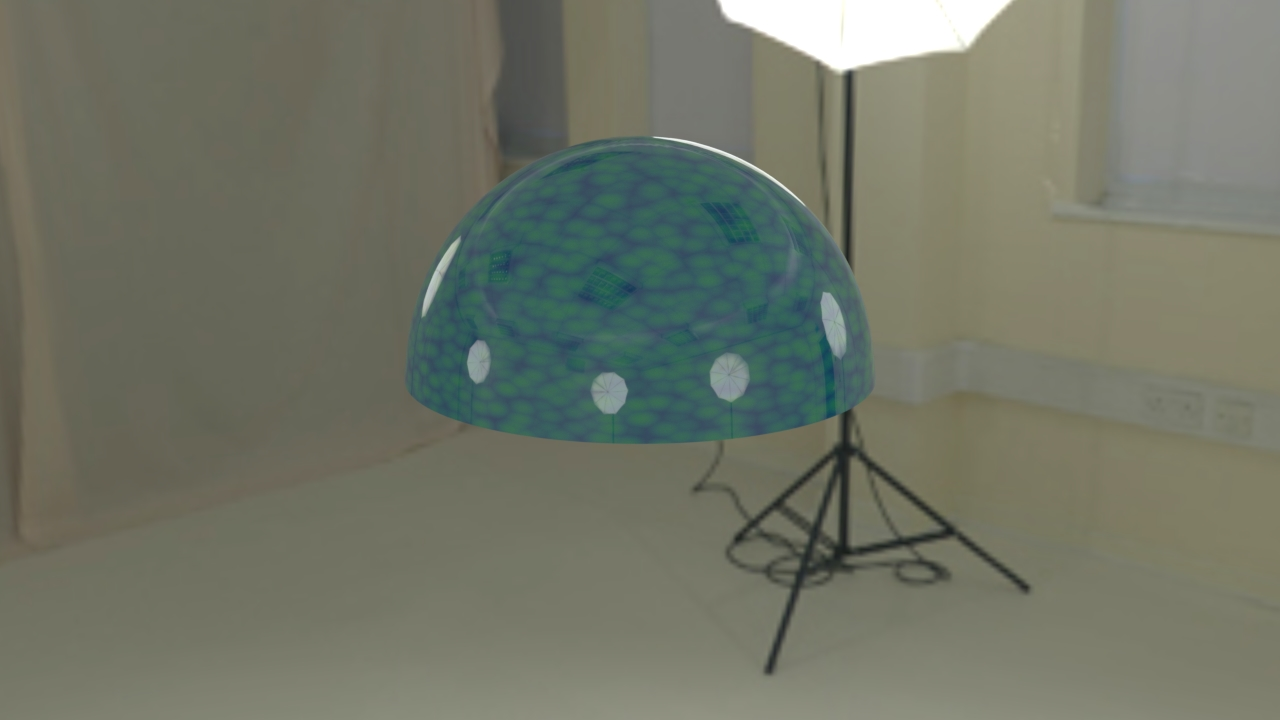
\includegraphics[width=0.33\textwidth]{mapping/mvs_alb_spec/alb_spec_0502}&
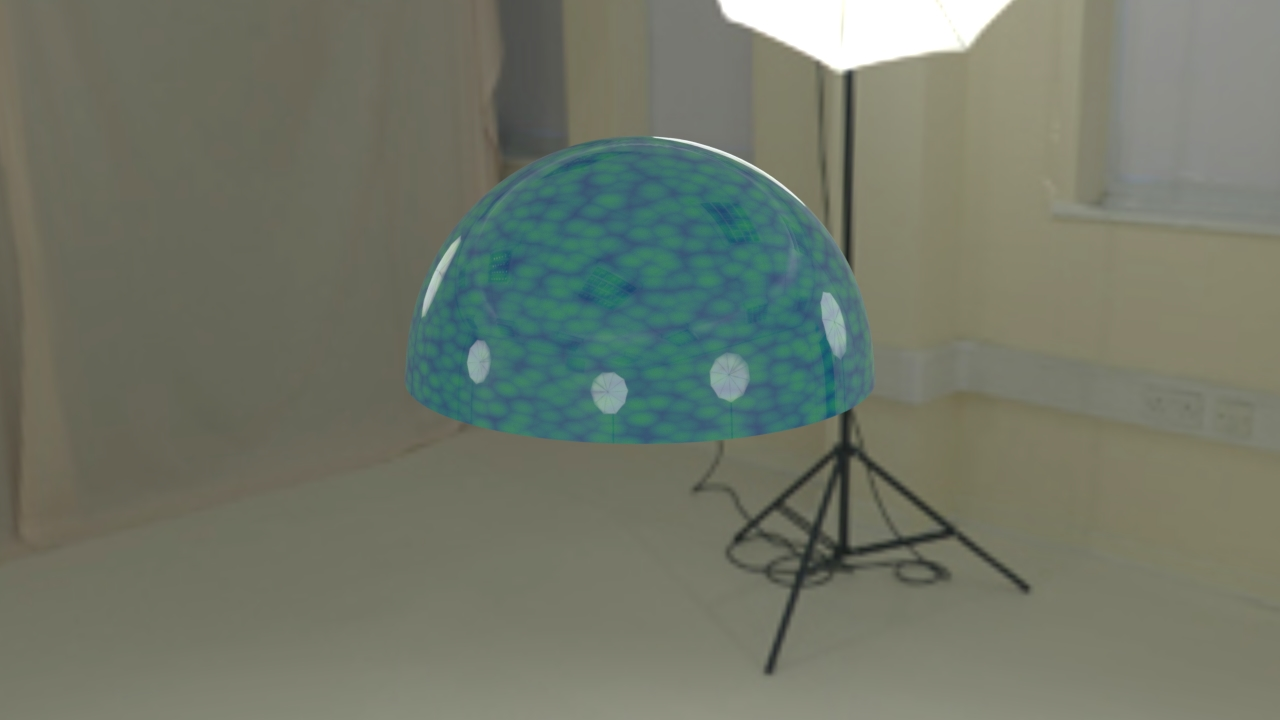
\includegraphics[width=0.33\textwidth]{mapping/mvs_alb_spec/alb_spec_0802}\\
(d) alb: 0.2 & (e) alb: 0.5 & (f) alb: 0.8\\
\end{tabular}
\caption{(a)-(c). The albedo is set as 0.2, (d)-(f). the specular is set as 0.2. According to energy conservation, as the specular component increases, the diffuse component decreases.}
\label{fig:mvs_alb_spec}
\end{figure}

\textbf{(f) Specular and Roughness} 
The effect of roughness is that it can diminish the specular and make the surface appearch diffuse. Since specular has a negative impact on the reconstruction, in theory, roughness should have a positive impact on the reconstruction. However, since this test is conducted on highly textured surface, as shown before, the reconstruction is still good for specular, highly textured surface, refer to~\ref{fig:mvs_depend_check}(b). That's why the effect of roughness on specualar seem insignificant. Since for this method, these two property are closed related, we'll just consider specular only, and ignore roughness. since a low specular achieve almost the same result as a high specular and rough surface, we would just combine these two factors into a single one, and consider the specular only for simplicity.

\textbf{Conclusion} 
The most important property is, high texture would lead to good reconstruction. Specular effect would deteriorate the reconstruction for lower textured and lower albedo surfaces. Since low specular and high specular + rough achieves almost the same results, we combine these two factors together and consider specular only.

the properties that have an effect on the MVS are: texture, albedo, and specularity, as shown in Table~\ref{tab:mvs_depend_prop}. Thus, we will only consider these three properties for all forthcoming discussion of MVS.
\begin{table}[!htbp]
  \centering
  \begin{tabular}{l*{4}{c}}
  \hline
  \textbf{Metric} & Texture & Albedo & Specular & Roughness\\
  \hline
  Accuracy & \ding{55} & \checkmark & \checkmark & \ding{55}\\
  Completeness & \checkmark & \checkmark & \checkmark & \ding{55}\\
  \hline
  \end{tabular}
  \caption{The correlation between each property and the metrics \textit{accuracy} and \textit{completeness}.}
  \label{tab:mvs_depend_prop}
\end{table}

% \begin{table}[!htbp]
%   % \centering
%   \begin{tabular}{*{4}{c}r||*{4}{c}r||*{4}{c}r}
%   \hline
%   T & A & S & R & RS & T & A & S & R & RS & T & A & S & R & RS\\
%   \hline
%   0.2 & 0.2 & 0.2 & 0.0 & \ding{55} & 0.5 & 0.2 & 0.2 & 0.0 & \ding{55} & 0.8 & 0.2 & 0.2 & 0.0 & \ding{55}\\
%   0.2 & 0.2 & 0.5 & 0.0 & \ding{55} & 0.5 & 0.2 & 0.5 & 0.0 & \ding{55} & 0.8 & 0.2 & 0.5 & 0.0 & \ding{55}\\
%   0.2 & 0.2 & 0.8 & 0.0 & \ding{55} & 0.5 & 0.2 & 0.8 & 0.0 & \ding{55} & 0.8 & 0.2 & 0.8 & 0.0 & \ding{55}\\
%   0.2 & 0.5 & 0.2 & 0.0 & \ding{55} & 0.5 & 0.5 & 0.2 & 0.0 & \ding{55} & 0.8 & 0.5 & 0.2 & 0.0 & \ding{55}\\
%   0.2 & 0.5 & 0.5 & 0.0 & \ding{55} & 0.5 & 0.5 & 0.5 & 0.0 & \ding{55} & 0.8 & 0.5 & 0.5 & 0.0 & \ding{55}\\
%   0.2 & 0.5 & 0.8 & 0.0 & \ding{55} & 0.5 & 0.5 & 0.8 & 0.0 & \ding{55} & 0.8 & 0.5 & 0.8 & 0.0 & \ding{55}\\
%   0.2 & 0.8 & 0.2 & 0.0 & \ding{55} & 0.5 & 0.8 & 0.2 & 0.0 & \ding{55} & 0.8 & 0.8 & 0.2 & 0.0 & \ding{55}\\
%   0.2 & 0.8 & 0.5 & 0.0 & \ding{55} & 0.5 & 0.8 & 0.5 & 0.0 & \ding{55} & 0.8 & 0.8 & 0.5 & 0.0 & \ding{55}\\
%   0.2 & 0.8 & 0.8 & 0.0 & \ding{55} & 0.5 & 0.8 & 0.8 & 0.0 & \ding{55} & 0.8 & 0.8 & 0.8 & 0.0 & \ding{55}\\
%   \hline
%   \end{tabular}
%   \caption{Mapping from the problem conditions to PMVS}
% \end{table}

\subsection{Example-based PS}
We evaluate the performance of example-based PS in terms of angular difference under varied combinations of properties, The statistical measures that we used include median, mean, first and third quartile of the angular difference. We investigate two properties at a time. The settings of the properties and all their combinations are listed in Table~\ref{tab:ps_depend_check_params}.

\begin{table}[!htbp]
  \centering
  \begin{tabular}{l*{4}{c}}
  \hline
  \textbf{Property} & Texture & Albedo & Specular & Roughness\\
  \hline
  \textbf{(a)} & [0.2, 0.8] & [0.2, 0.8] & 0.0 & 0.0\\
  \textbf{(b)} & [0.2, 0.8] & 0.8 & [0.2, 0.8] & 0.2\\
  \textbf{(c)} & [0.2, 0.8] & 0.8 & 0.0 & [0.2, 0.8]\\
  \textbf{(d)} & 0.0 & [0.2, 0.8] & [0.2, 0.8] & 0.2\\
  \textbf{(e)} & 0.0 & [0.2, 0.8] & 0.0 & [0.2, 0.8]\\
  \textbf{(f)} & 0.0 & 0.8 & [0.2, 0.8] & [0.2, 0.8]\\
  \hline
  \end{tabular}
  \caption{Property settings of the pairwise conditions used for the dependency check of the Photometric Stereo algorithms.}
  \label{tab:ps_depend_check_params}
\end{table}

\begin{figure}[!htbp]
\begin{tabular}{cc}
\includegraphics[width=0.5\textwidth]{mapping/depend_check/ps_tex_alb}&
\includegraphics[width=0.5\textwidth]{mapping/depend_check/ps_tex_spec}\\
(a) & (b)\\
\includegraphics[width=0.5\textwidth]{mapping/depend_check/ps_tex_rough}&
\includegraphics[width=0.5\textwidth]{mapping/depend_check/ps_alb_spec}\\
(c) & (d)\\
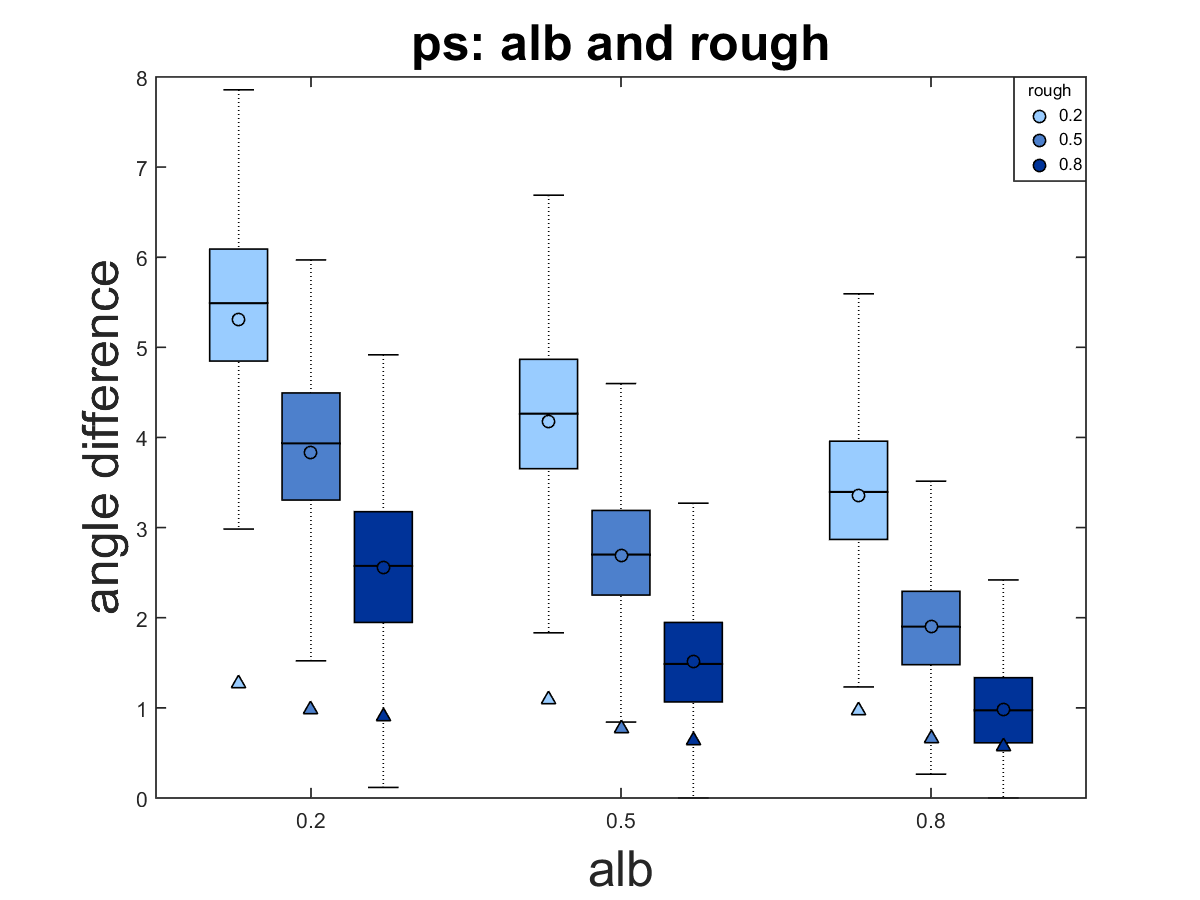
\includegraphics[width=0.5\textwidth]{mapping/depend_check/ps_alb_rough}&
\includegraphics[width=0.5\textwidth]{mapping/depend_check/ps_spec_rough}\\
(e) & (f)\\
\end{tabular}
\caption{Performance of Example-based PS under six pairwise conditions. For instance, (a) shows the performance under changing \textit{texture} and \textit{albedo} values. The property values are assigned based on Table~\ref{tab:ps_depend_check_params} (a).}
\label{fig:ps_depend_check}
\end{figure}

\subsection{Single property}
\textbf{Texture} - \textit{(a), (b), (c)}. As the texture level increases, all statistic measures of the angular difference remain almost the same. Thus texture doesn't affect the reconstruction of the chosen PS algorithm.

\textbf{Albedo} - \textit{(a), (d), (e)}. As the albedo level increases, all statistic measures of the angular difference decreases. Thus the albedo has a positive correlation to the reconstruction.

\textbf{Specular} - \textit{(b), (d), (f)}. As the specular level goes up, all statistic measures of the angular difference increases. Thus specular has an negative impact on the reconstruction.

\textbf{Roughness} - \textit{(c), (e), (f)}. The effect of roughness is a bit complicated. Generally, it will improve the reconstruction as the roughness goes higher. However, as shown in Figure~\ref{fig:ps_depend_check} (f), the roughness will cause worse reconstruction for medium high value, which will be discussed more later. As the surface roughness increases, the size of the highlight increases, making elimination of specularity harder. However, if the roughness increases enough, the surface begins to look diffuse.

\subsection{Pairwise properties}
All the pairwise relations are straightforward except for (f).

\textbf{(b) Texture and Specular}
\begin{figure}[!htbp]
\centering
\begin{tabular}{ccc}
\includegraphics[width=0.33\textwidth]{mapping/ps_tex_spec/0502_0001}&
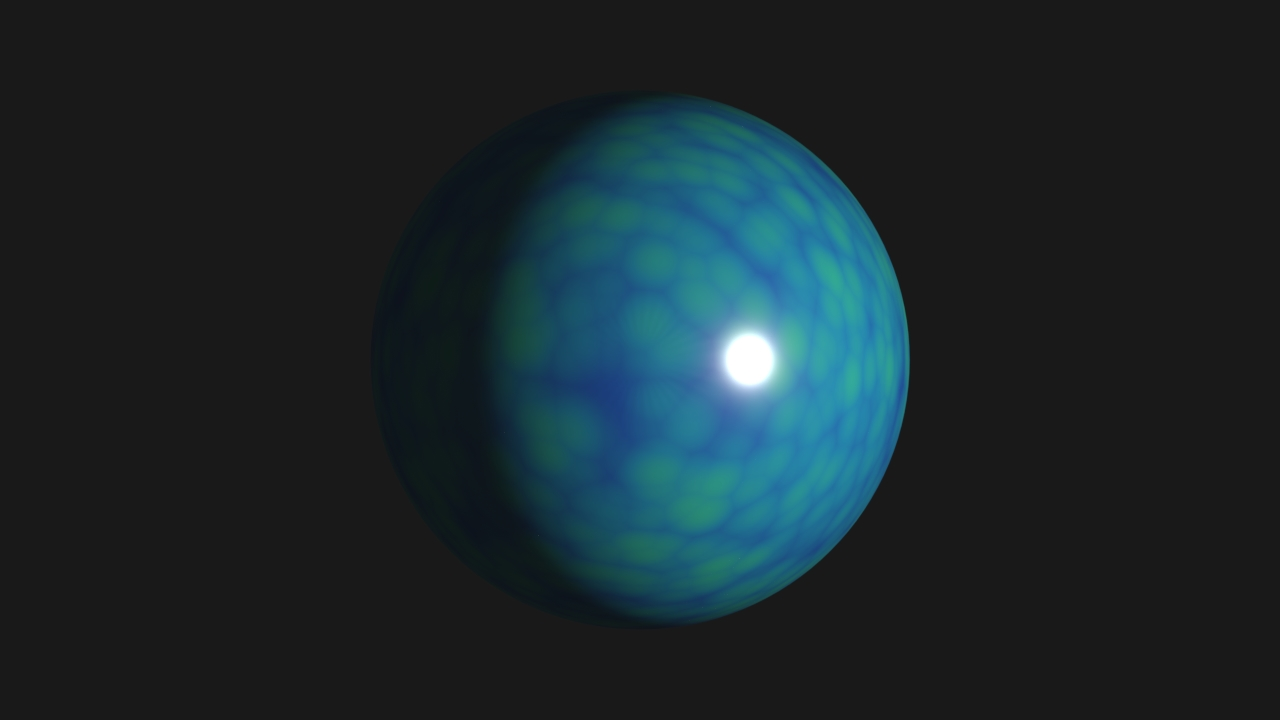
\includegraphics[width=0.33\textwidth]{mapping/ps_tex_spec/0505_0001}&
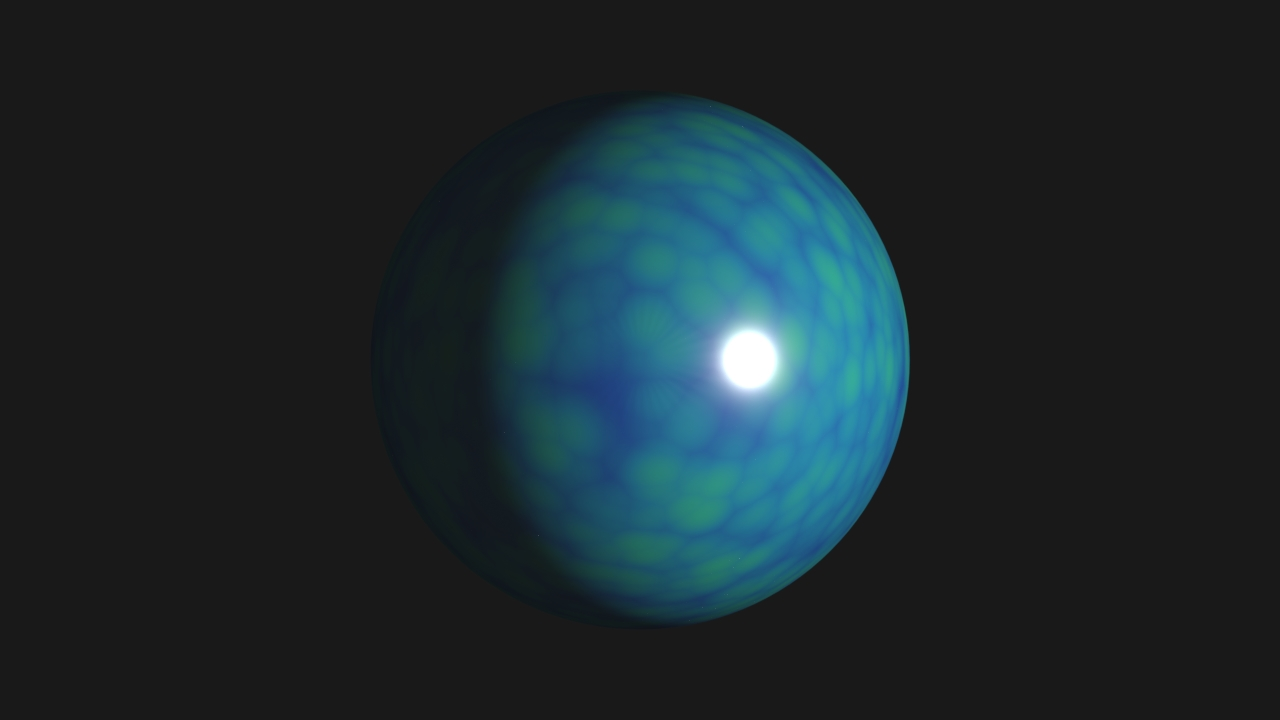
\includegraphics[width=0.33\textwidth]{mapping/ps_tex_spec/0508_0001}\\
\includegraphics[width=0.33\textwidth]{mapping/ps_tex_spec/0502_normal}&
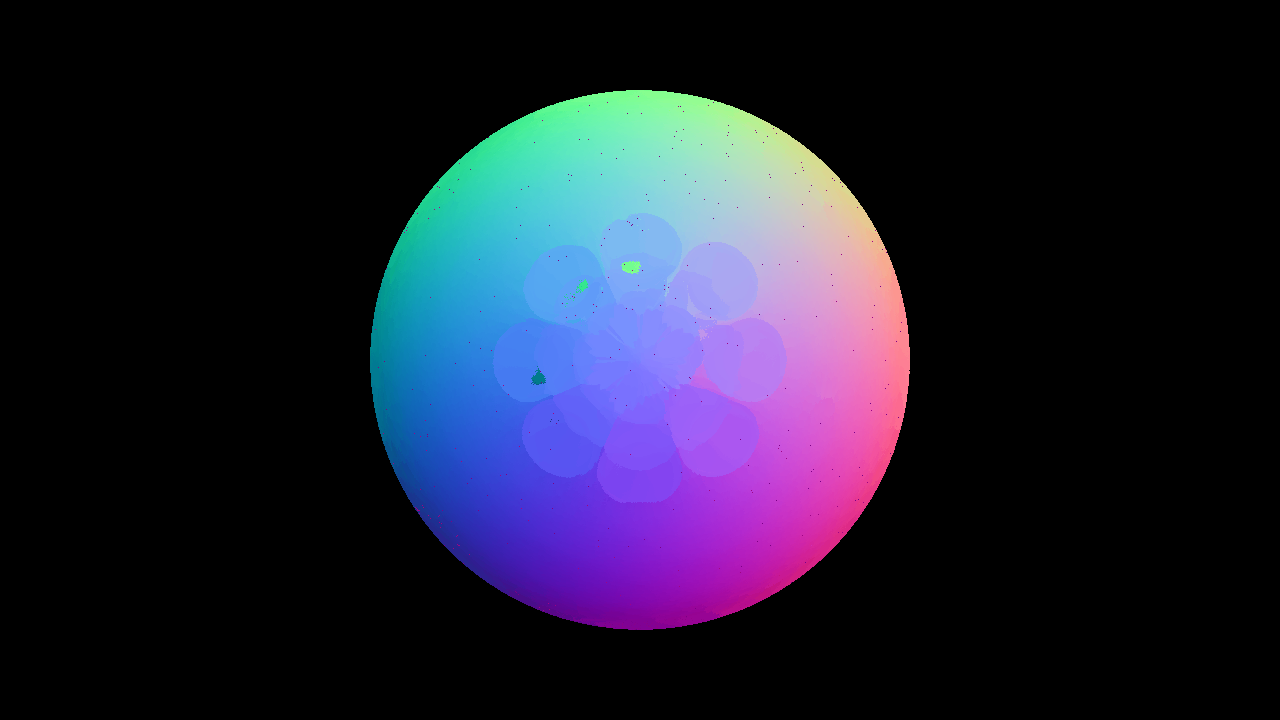
\includegraphics[width=0.33\textwidth]{mapping/ps_tex_spec/0505_normal}&
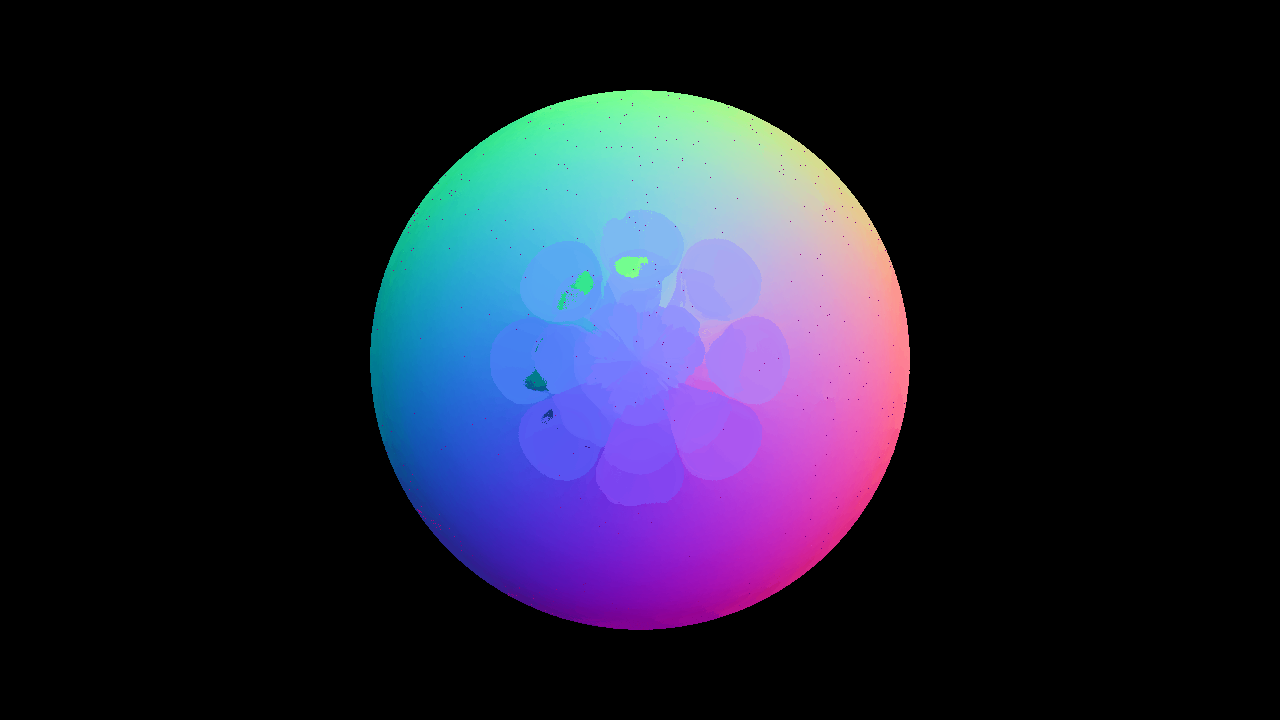
\includegraphics[width=0.33\textwidth]{mapping/ps_tex_spec/0508_normal}\\
(a) spec: 0.2 & (b) spec: 0.5 & (c) spec: 0.8\\
\end{tabular}
\caption{(a)-(c). The texture is set as 0.5. According to energy conservation, as the specular component increases, the diffuse component decreases.}
\label{fig:mvs_alb_spec}
\end{figure}

\textbf{(b) Albedo and Specular}
For 
\begin{figure}[!htbp]
\centering
\begin{tabular}{ccc}
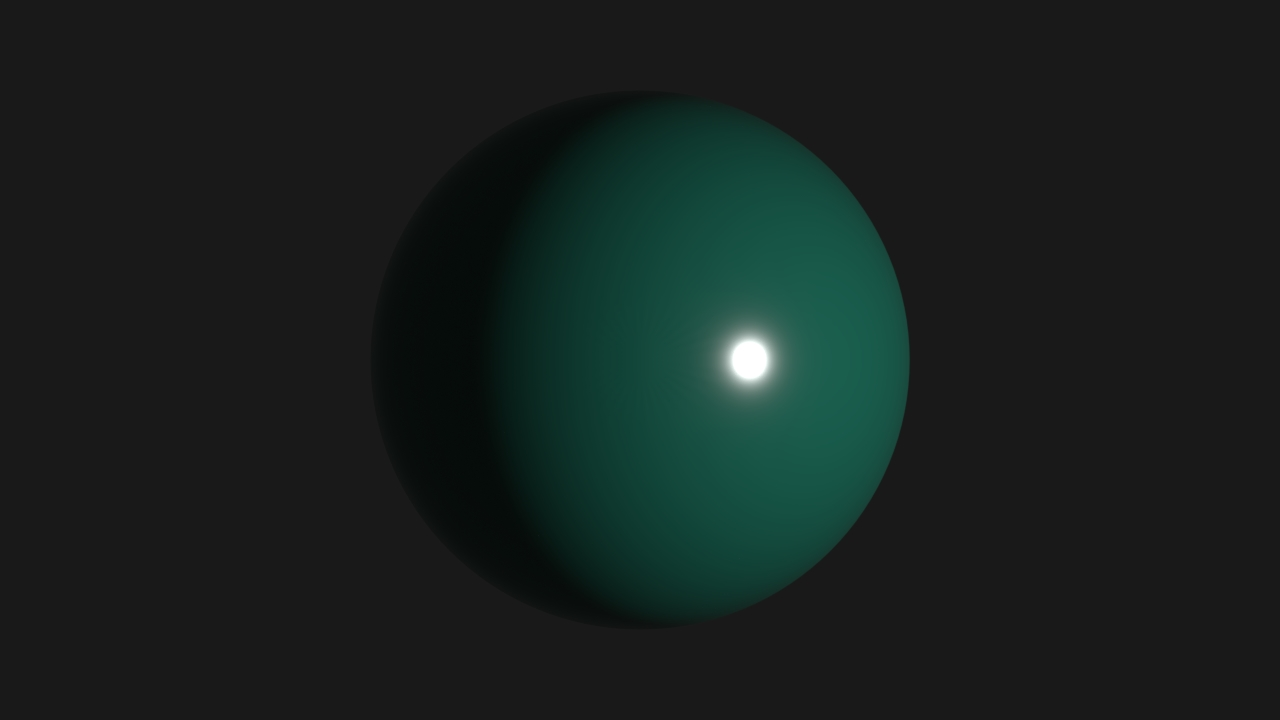
\includegraphics[width=0.33\textwidth]{mapping/ps_alb_spec/0202_0001}&
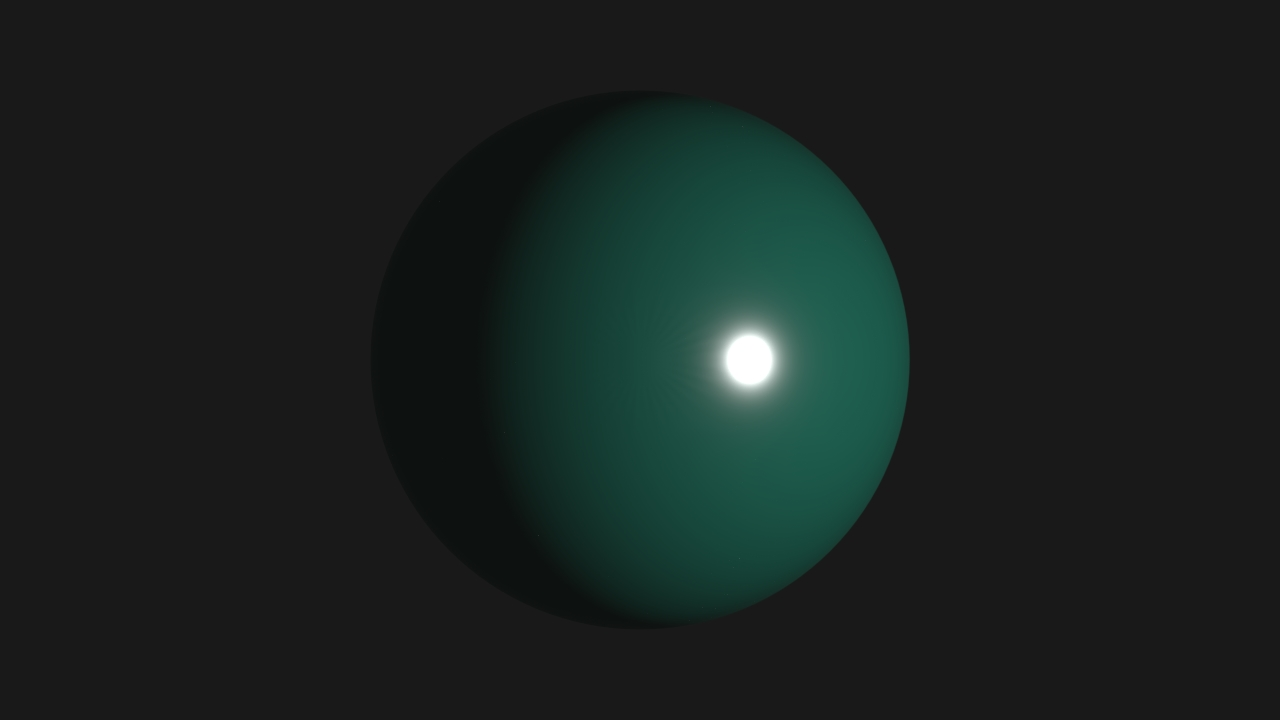
\includegraphics[width=0.33\textwidth]{mapping/ps_alb_spec/0205_0001.jpg}&
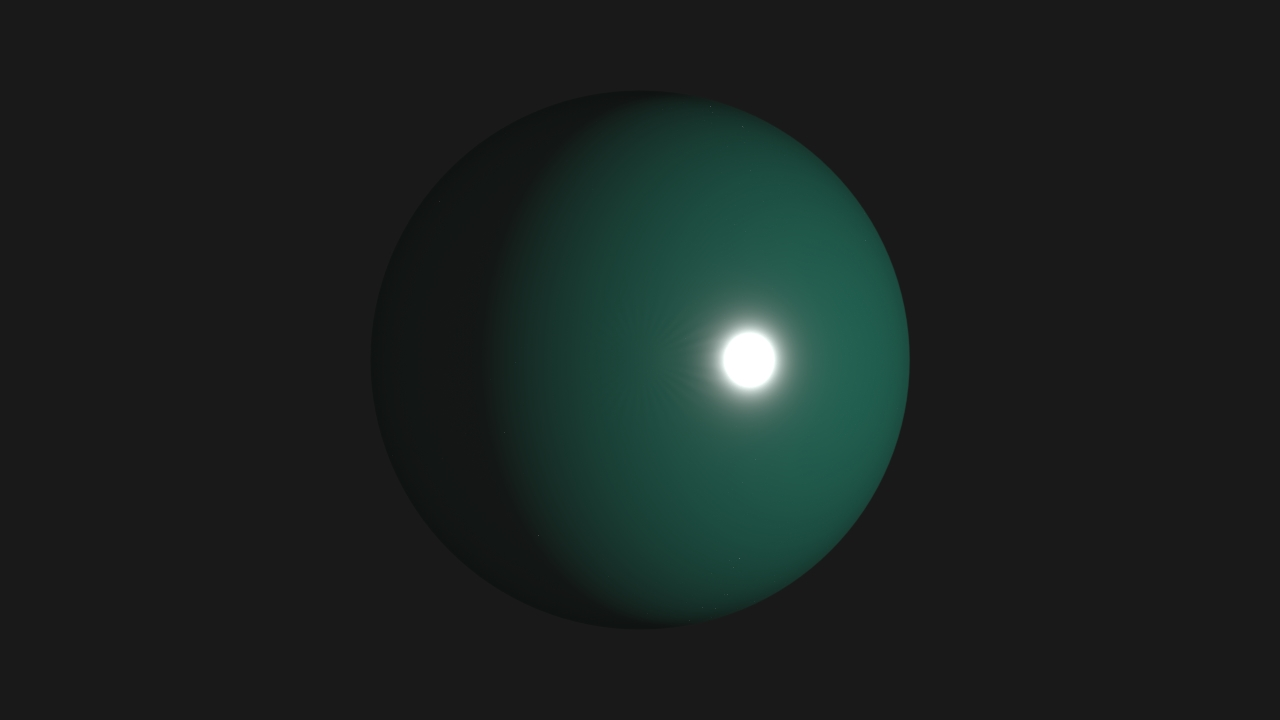
\includegraphics[width=0.33\textwidth]{mapping/ps_alb_spec/0208_0001}\\
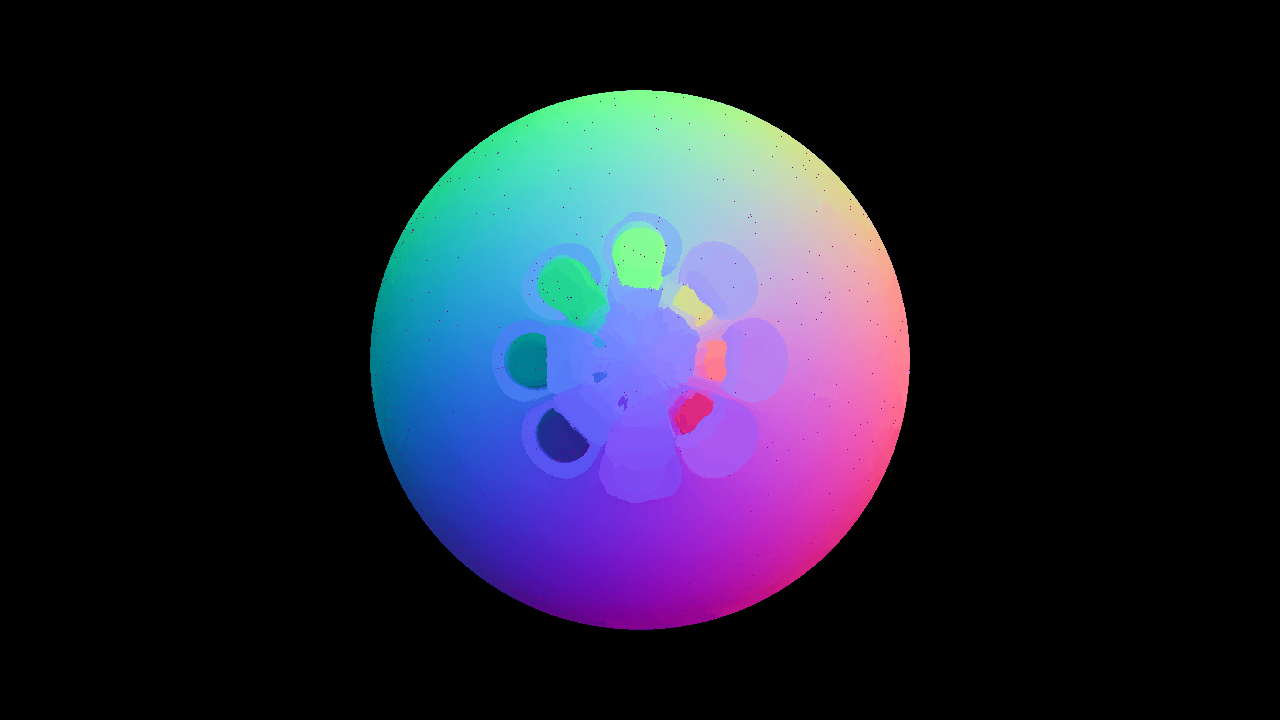
\includegraphics[width=0.33\textwidth]{mapping/ps_alb_spec/0202_normal}&
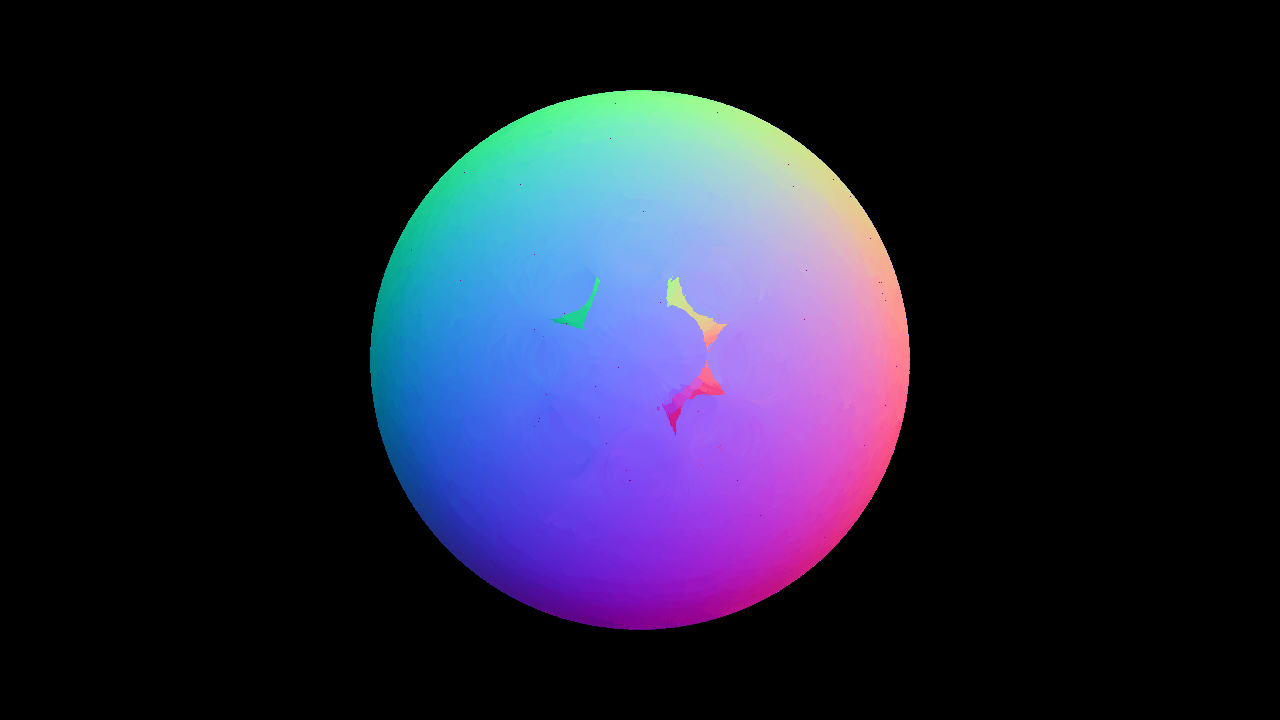
\includegraphics[width=0.33\textwidth]{mapping/ps_alb_spec/0205_normal.png}&
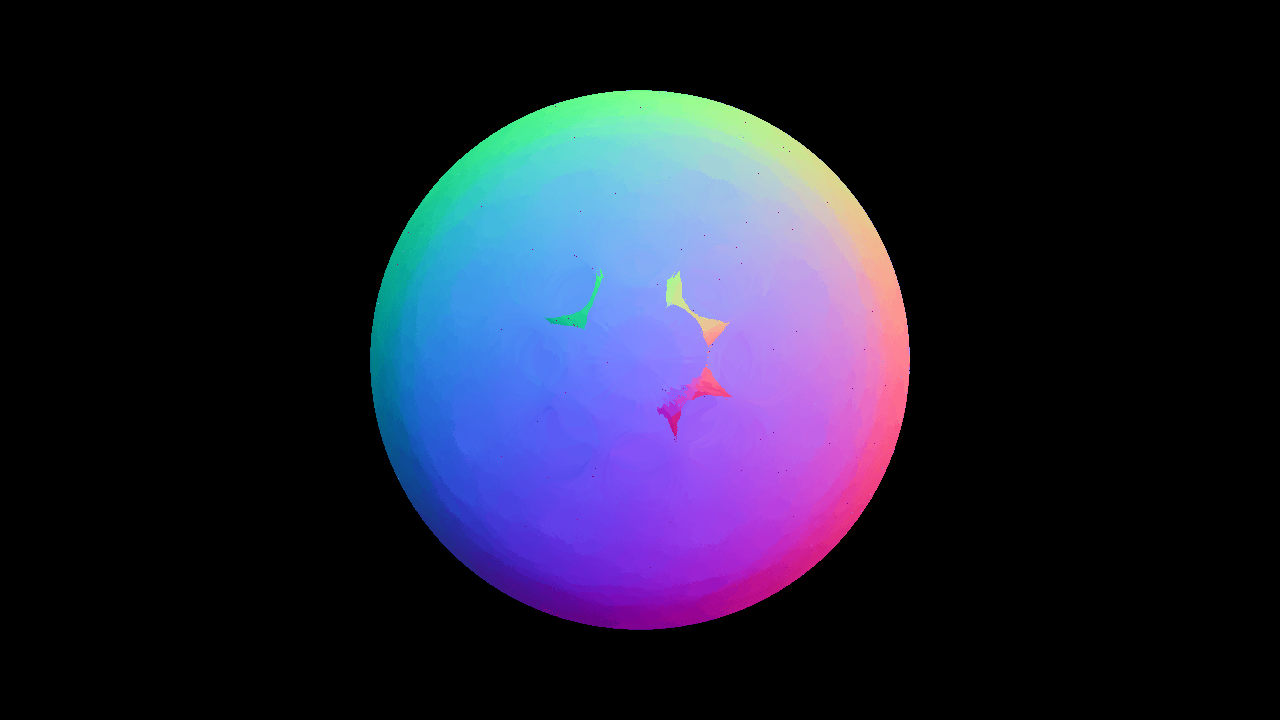
\includegraphics[width=0.33\textwidth]{mapping/ps_alb_spec/0208_normal}\\
(a) specular: 0.2 & (b) specular: 0.5 & (c) specular: 0.8\\
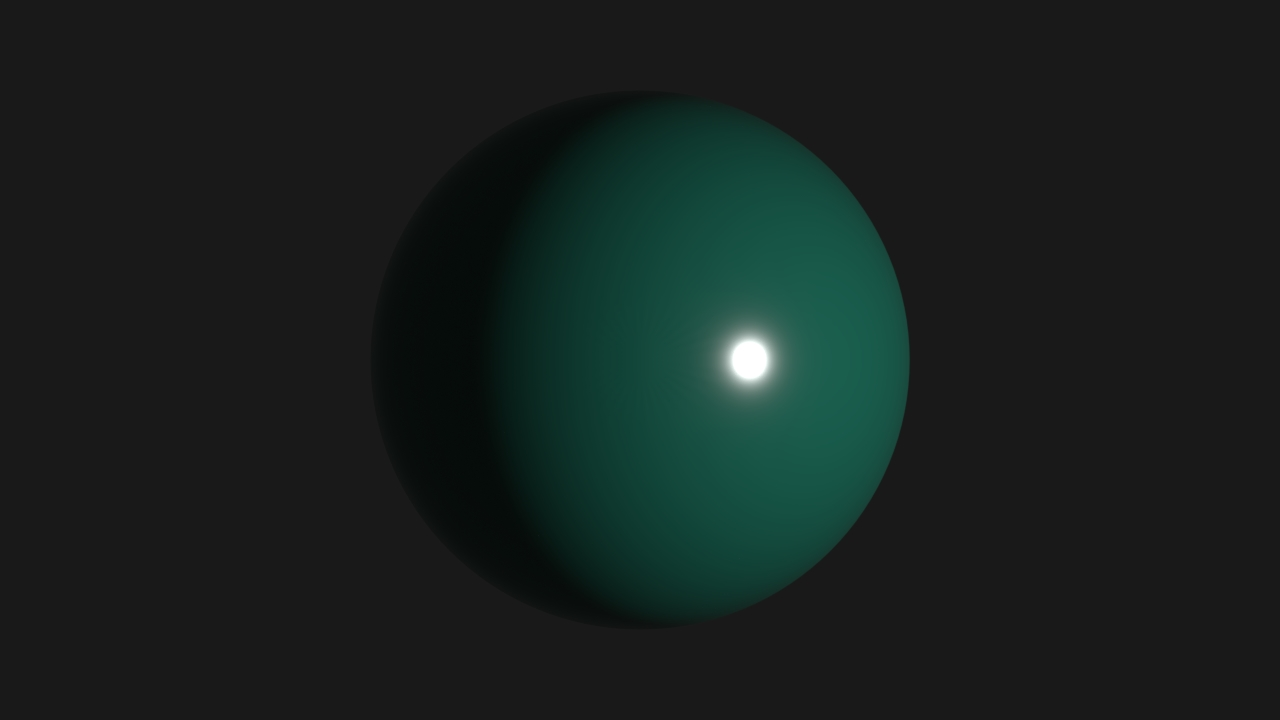
\includegraphics[width=0.33\textwidth]{mapping/ps_alb_spec/0202_0001}&
\includegraphics[width=0.33\textwidth]{mapping/ps_alb_spec/0502_0001}&
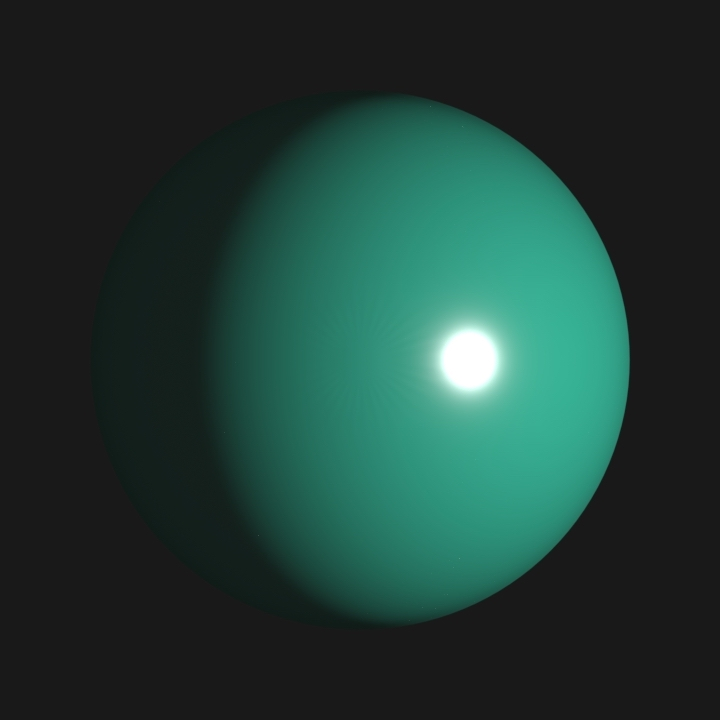
\includegraphics[width=0.33\textwidth]{mapping/ps_alb_spec/0802_0001}\\
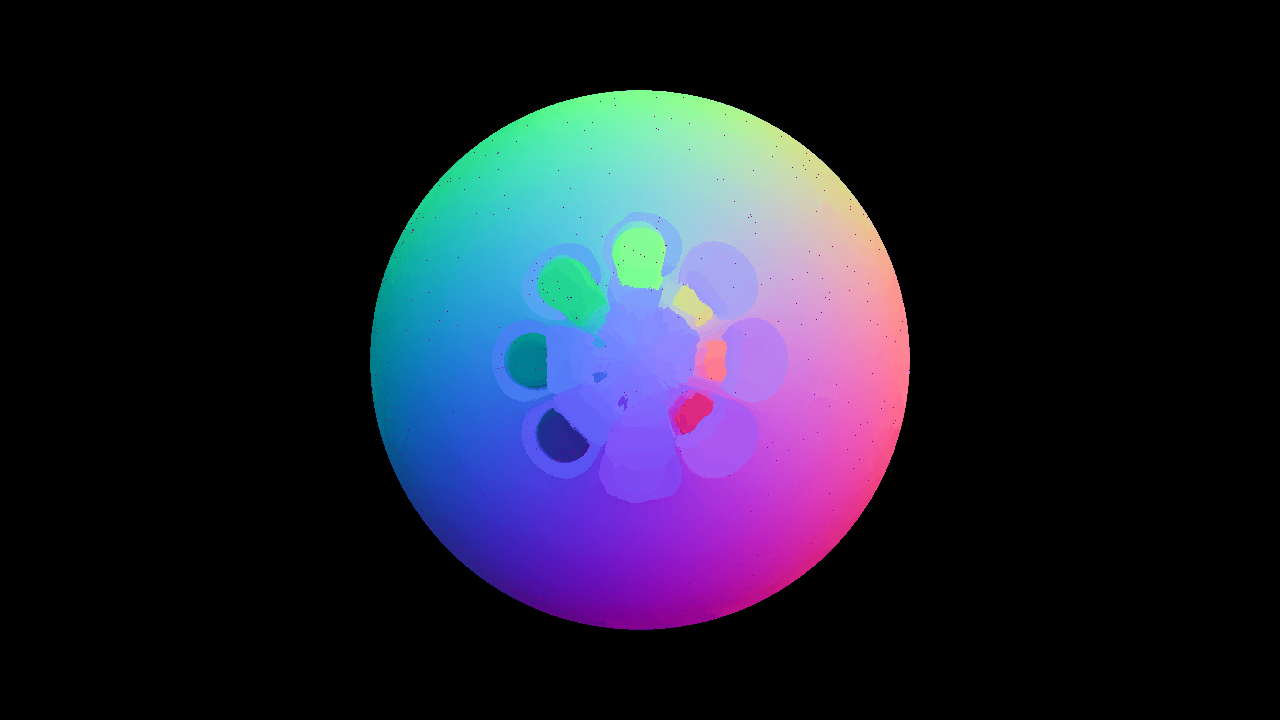
\includegraphics[width=0.33\textwidth]{mapping/ps_alb_spec/0202_normal}&
\includegraphics[width=0.33\textwidth]{mapping/ps_alb_spec/0502_normal}&
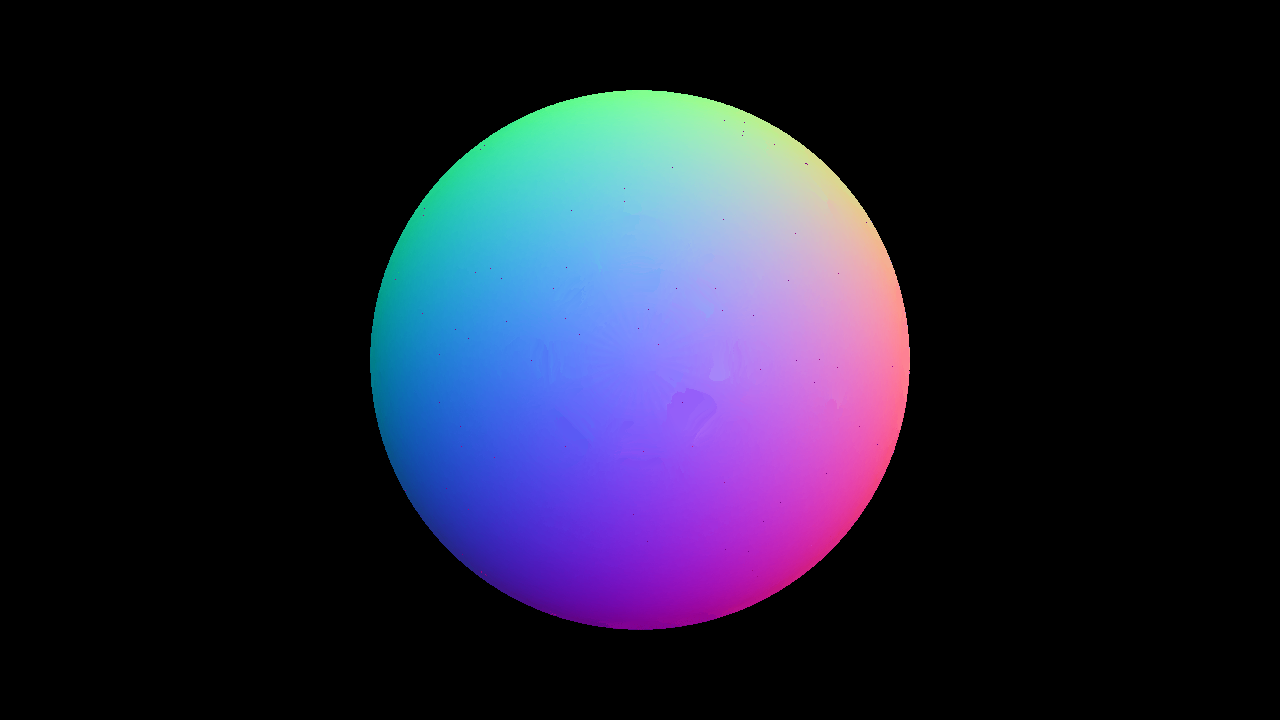
\includegraphics[width=0.33\textwidth]{mapping/ps_alb_spec/0802_normal}\\
(d) albedo: 0.2 & (e) albedo: 0.5 & (f) albedo: 0.8\\
\end{tabular}
\caption{(a)-(c). The albedo is set as 0.2, (d)-(f). the specular is set as 0.2. According to energy conservation, as the specular component increases, the diffuse component decreases.}
\label{fig:mvs_alb_spec}
\end{figure}

\textbf{(f) Specularity and Roughness} 
For a fixed specularity, if the specularity is lower, the effect of roughness is less noticeable, whereas if the specularity is higher, the effect of roughness becomes more substantial. We've also noticed a `peculiar' case when roughness is 0.5, it makes the reconstruction worse, which is counter-intuitive. However, we argue that it's because the roughness effect is not strong enough to cancel out the specularity, thus causing a much larger area of `blurred' specularity, which makes the reconstruction worse. This effect is also demonstrated in the training stage, see Figure~\ref{fig:ps_outlier} for some visual examples.
\begin{figure}[h!]
\centering
\begin{tabular}{ccc}
  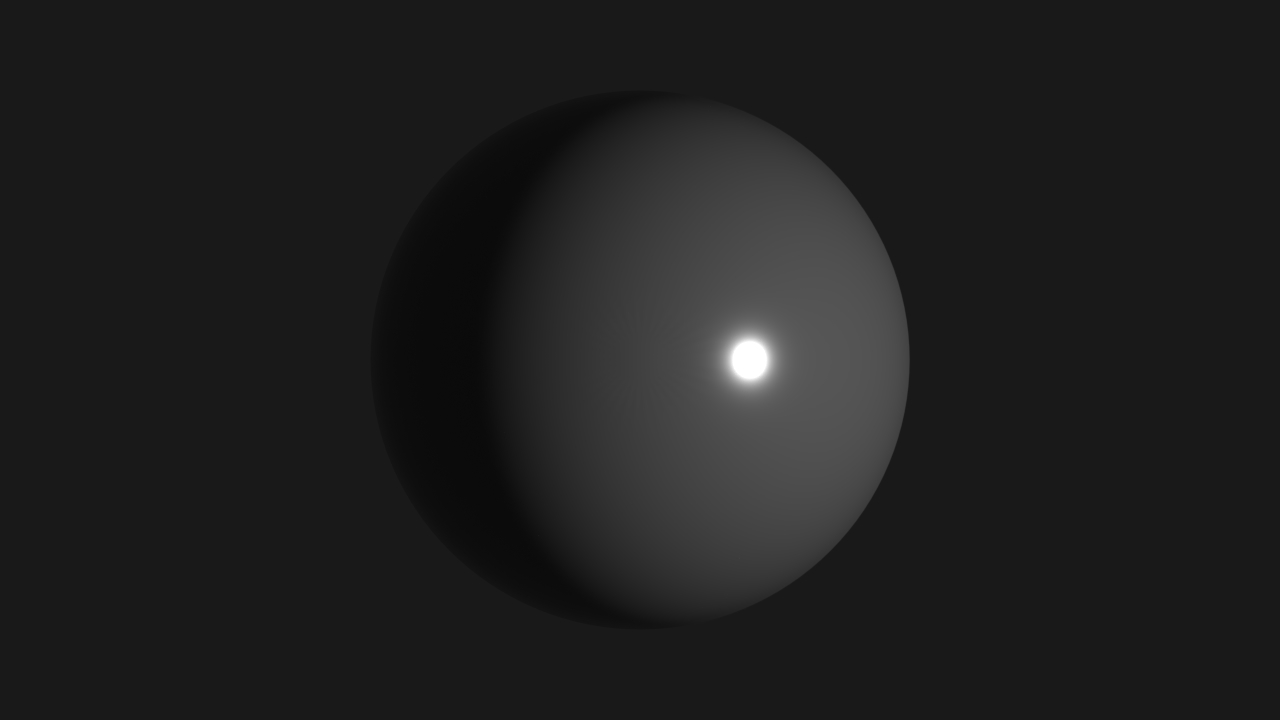
\includegraphics[width=0.35\textwidth]{mapping/ps_rough/00020202_0001}&
  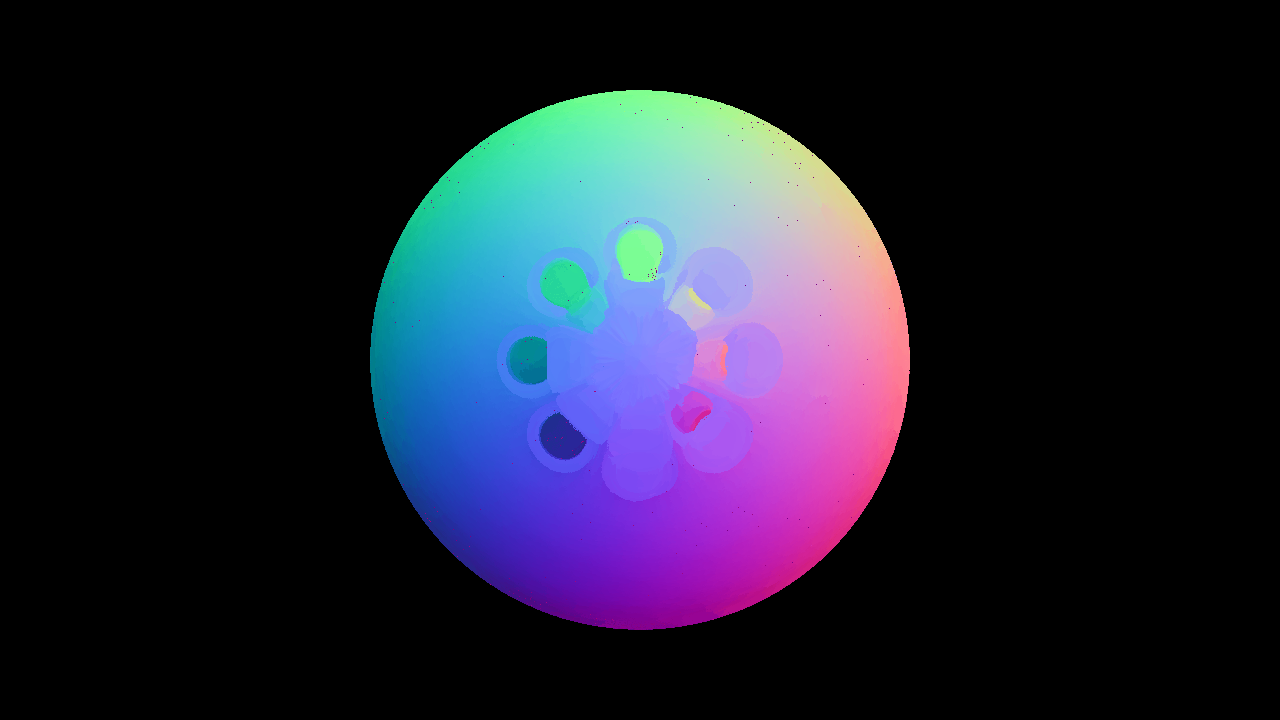
\includegraphics[width=0.35\textwidth]{mapping/ps_rough/00020202_normal}&
  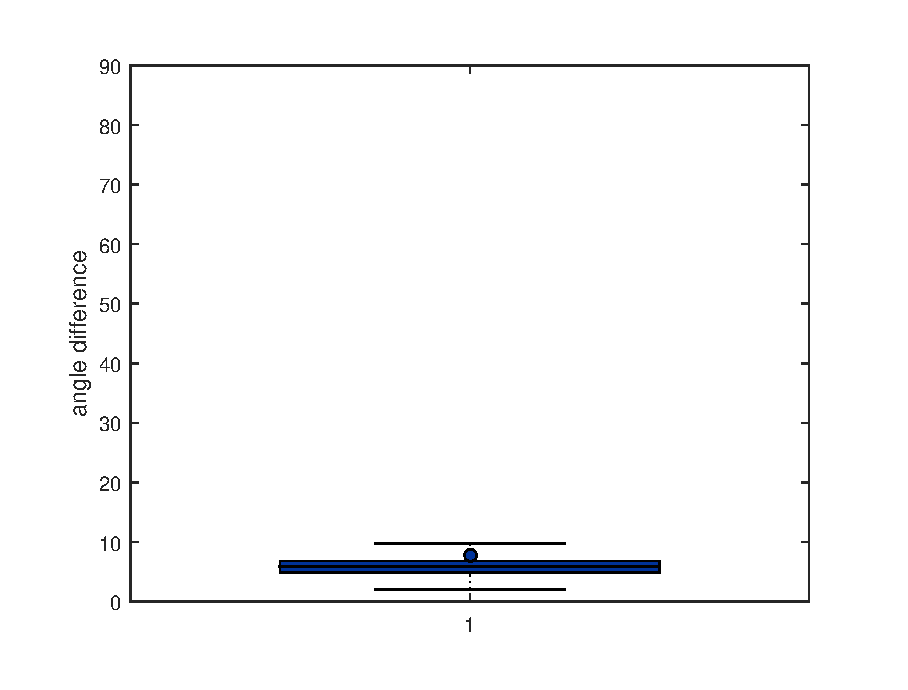
\includegraphics[width=0.30\textwidth]{mapping/ps_rough/00020202_boxplot}\\
  (a).020202 & (b). normal map & (c). angle diff distribution\\
  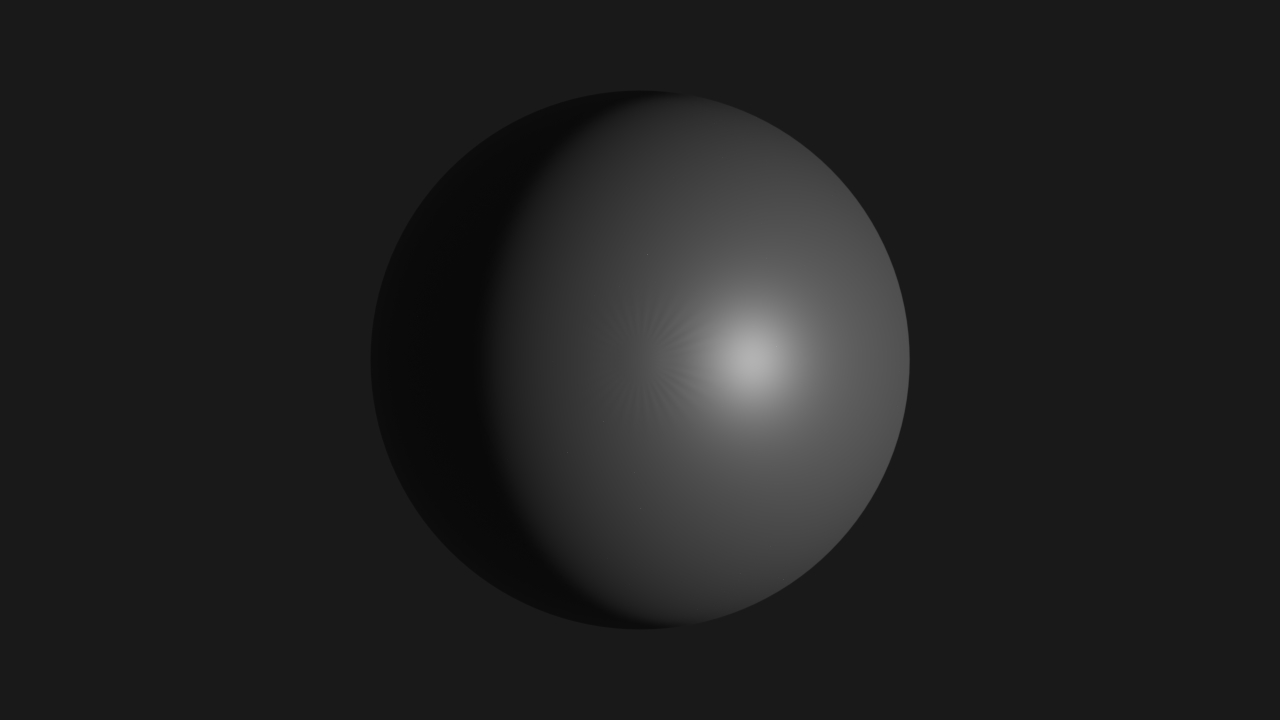
\includegraphics[width=0.35\textwidth]{mapping/ps_rough/00020205_0001}&
  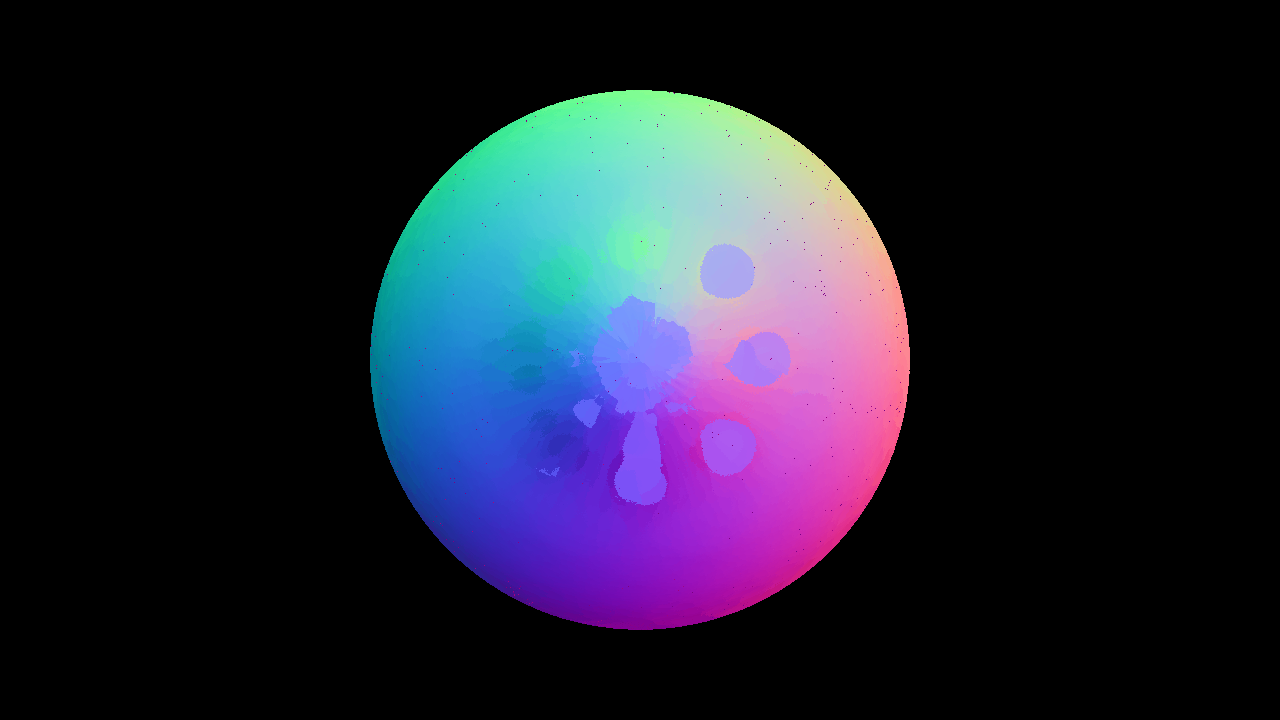
\includegraphics[width=0.35\textwidth]{mapping/ps_rough/00020205_normal}&
  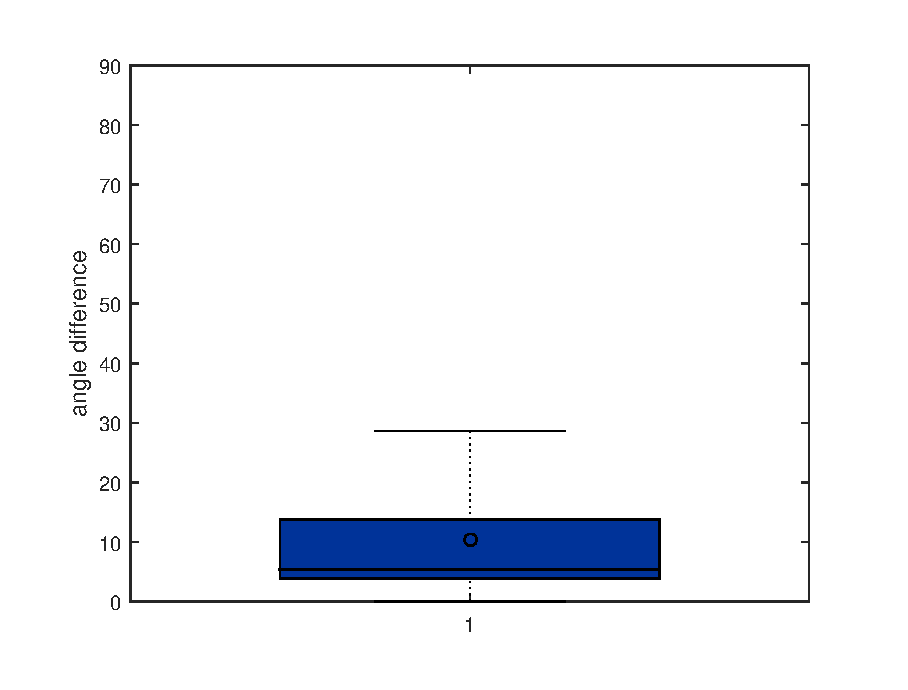
\includegraphics[width=0.30\textwidth]{mapping/ps_rough/00020205_boxplot}\\
  (d).020205 & (e). normal map & (f). angle diff distribution\\
  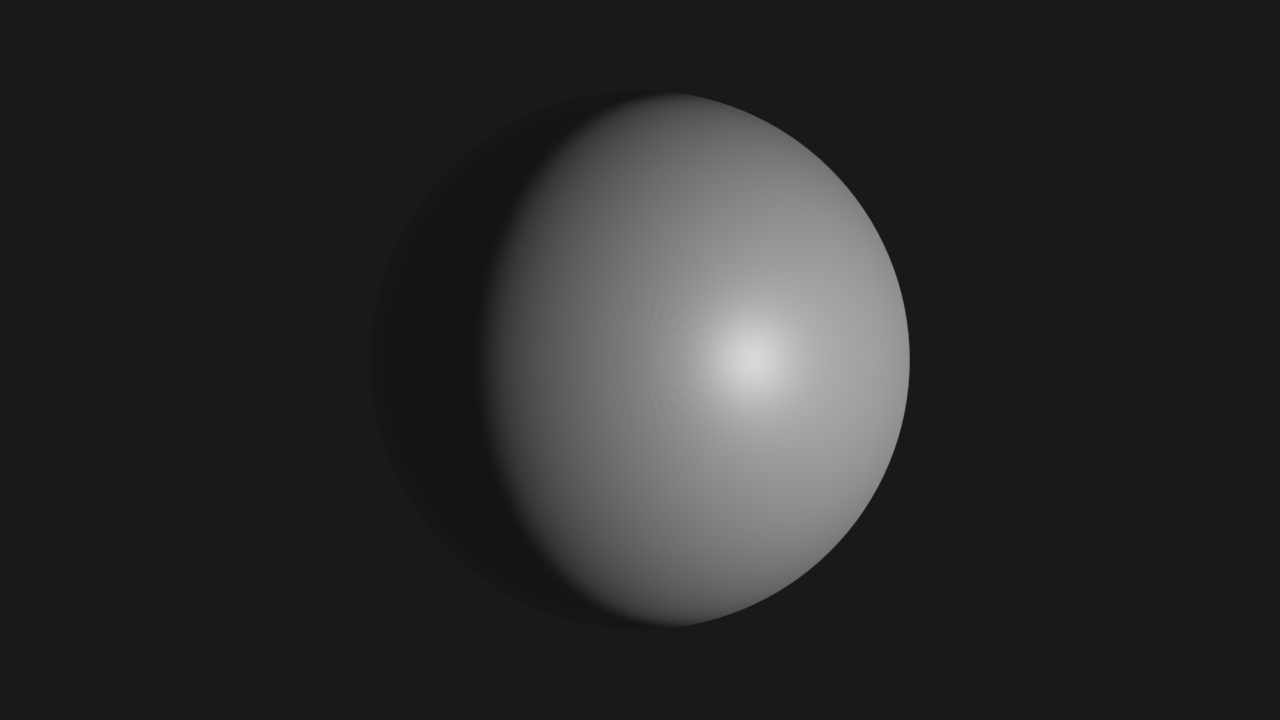
\includegraphics[width=0.35\textwidth]{mapping/ps_rough/00080205_0001}&
  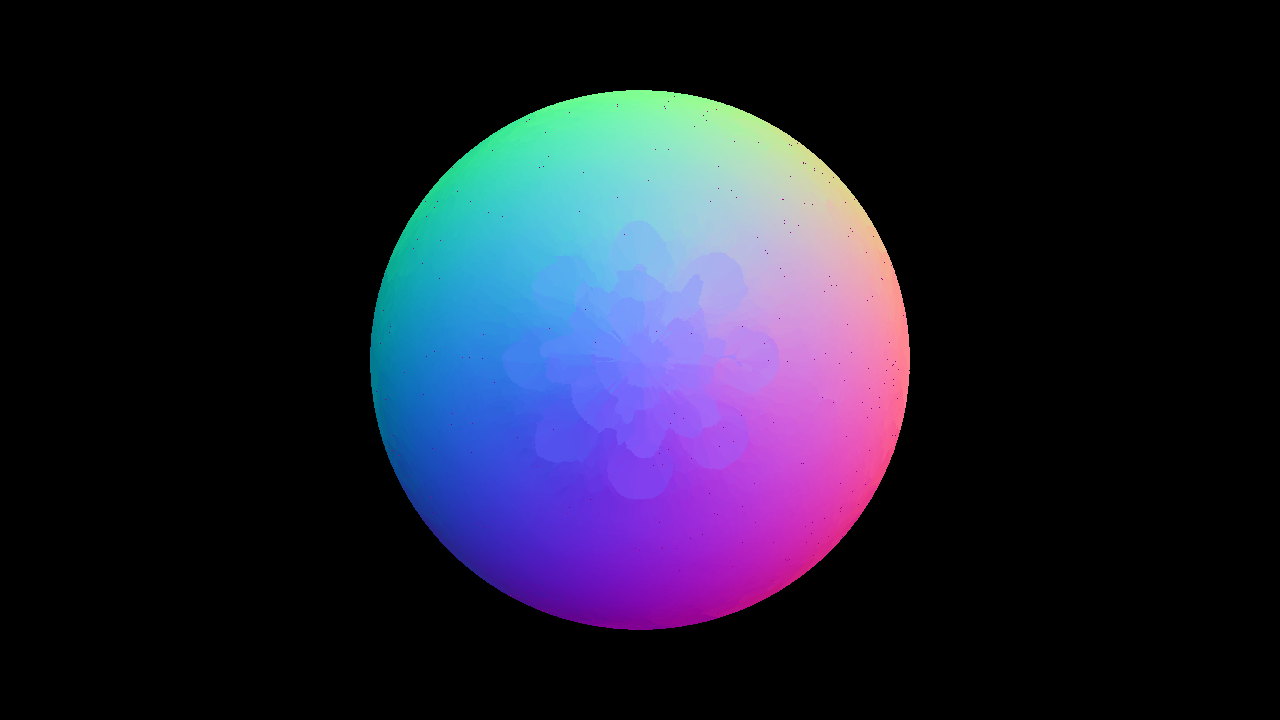
\includegraphics[width=0.35\textwidth]{mapping/ps_rough/00080205_normal}&
  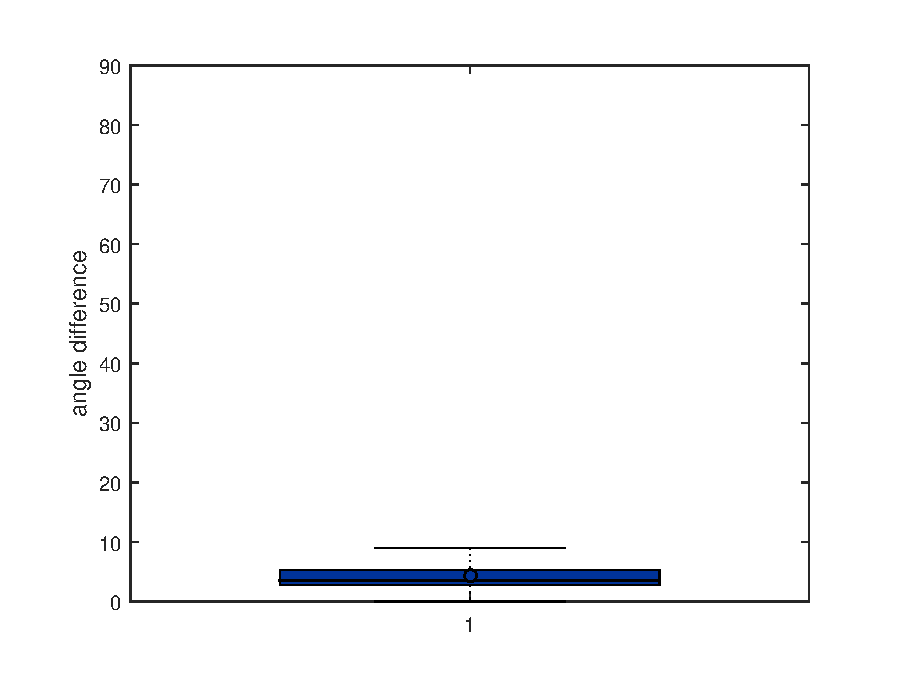
\includegraphics[width=0.30\textwidth]{mapping/ps_rough/00080205_boxplot}\\
  (g).080205 & (h). normal map & (i). angle diff distribution\\
  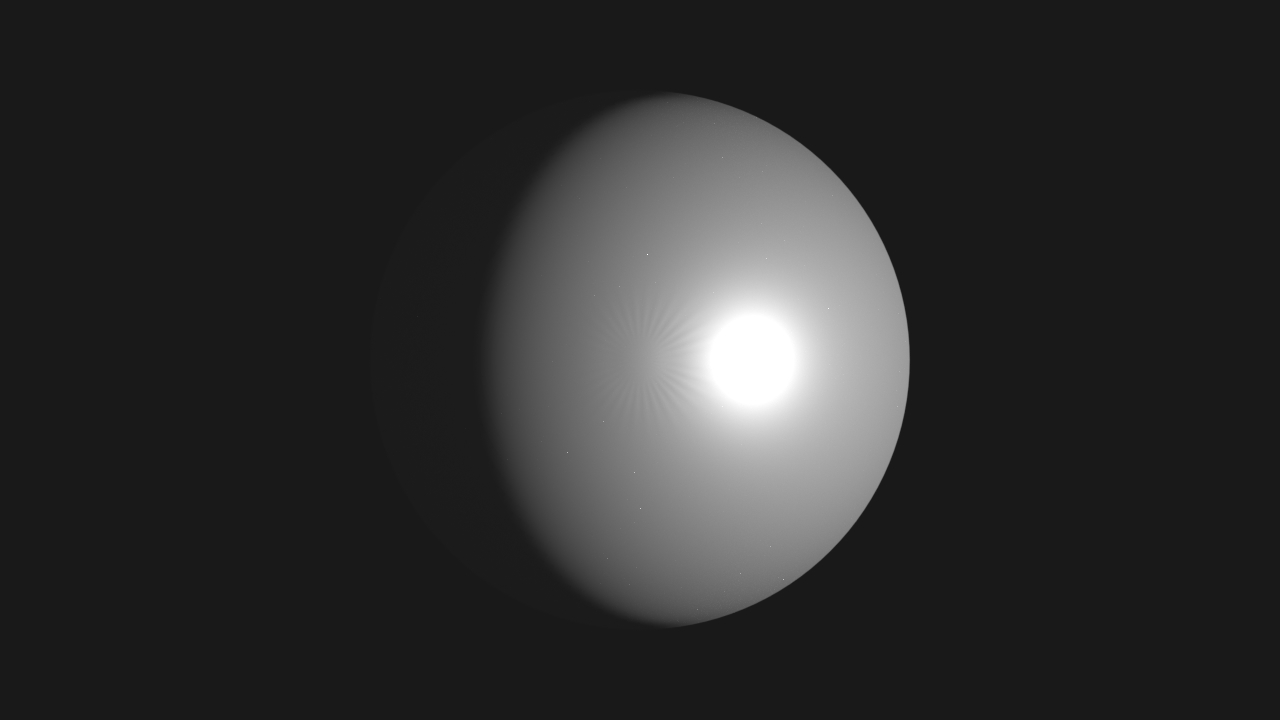
\includegraphics[width=0.35\textwidth]{mapping/ps_rough/00080805_0001}&
  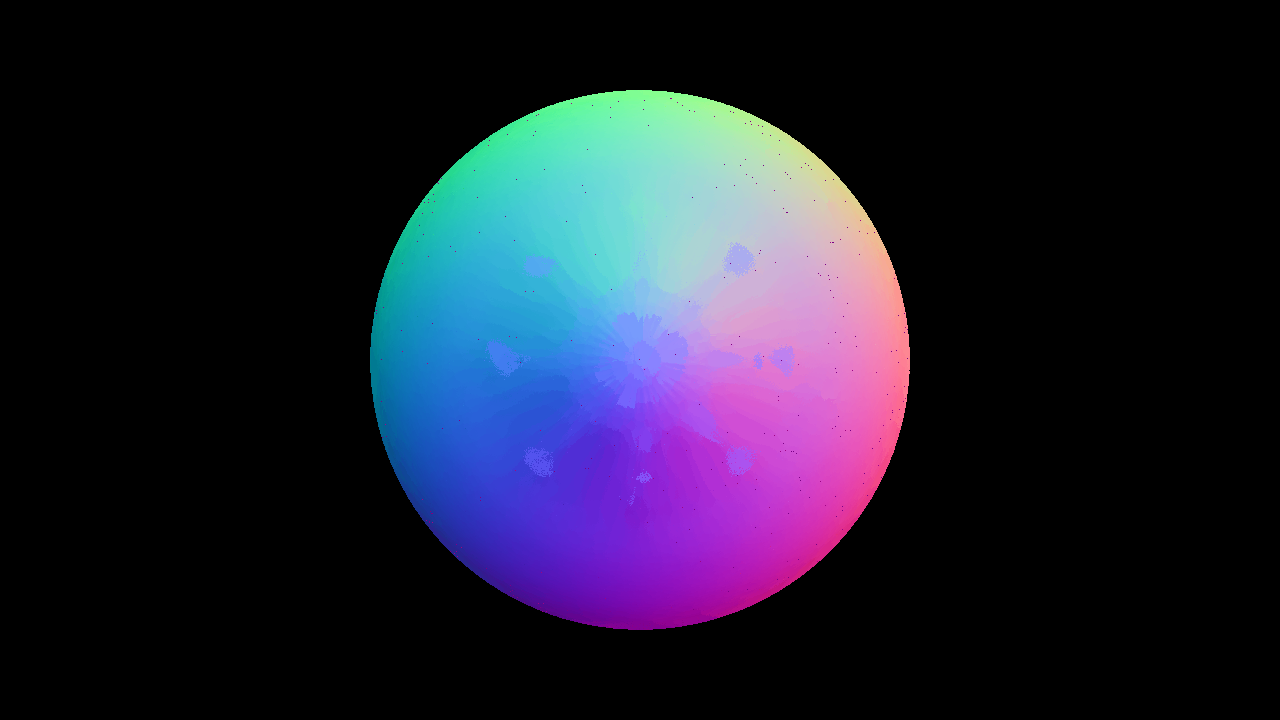
\includegraphics[width=0.35\textwidth]{mapping/ps_rough/00080805_normal}&
  \includegraphics[width=0.30\textwidth]{mapping/ps_rough/00080805_boxplot}\\
  (j).080805 & (k). normal map & (l). angle diff distribution\\
\end{tabular}
\caption{The `peculiar' effect of roughness on PS. The order of the property is: albedo, specular, and roughness, thus 080205 means albedo: 0.8, specular: 0.2, and roughness: 0.5}
\label{fig:ps_outlier}
\end{figure}

\textbf{Conclusion} the properties that have an effect on the PS are: albedo, specularity, and roughness, as shown in Table~\ref{tab:ps_depend_prop}. Therefore, we will only consider these three properties for all forthcoming discussion of PS.
\begin{table}[!htbp]
  \centering
  \begin{tabular}{l*{5}{c}}
  \hline
  \textbf{Metric} & Texture & Albedo & Specular & Roughness\\
  \hline
  Angle difference & \ding{55} & \checkmark & \checkmark & \checkmark\\
  \hline
  \end{tabular}
  \caption{The correlation between each property and the metric \textit{angular difference}.}
  \label{tab:ps_depend_prop}
\end{table}

\subsection{Gray-code SL}
We evaluate the performance of Gray-code SL in terms of accuracy and completeness under varied combination of properties, the settings of the properties and all their combinations are listed in Table~\ref{tab:sl_depend_check_params}.
\begin{table}[!htbp]
  \centering
  \begin{tabular}{l*{4}{c}}
  \hline
  \textbf{Property} & Texture & Albedo & Specular & Roughness\\
  \hline
  \textbf{(a)} & [0.2, 0.8] & [0.2, 0.8] & 0.0 & 0.0\\
  \textbf{(b)} & [0.2, 0.8] & 0.8 & [0.2, 0.8] & 0.0\\
  \textbf{(c)} & [0.2, 0.8] & 0.8 & 0.0 & [0.2, 0.8]\\
  \textbf{(d)} & 0.0 & [0.2, 0.8] & [0.2, 0.8] & 0.0\\
  \textbf{(e)} & 0.0 & [0.2, 0.8] & 0.0 & [0.2, 0.8]\\
  \textbf{(f)} & 0.0 & 0.8 & [0.2, 0.8] & [0.2, 0.8]\\
  \hline
  \end{tabular}
  \caption{Property settings of the pairwise conditions used for the dependency check of the Structured Light algorithms.}
  \label{fig:sl_depend_check_params}
\end{table}

\begin{figure}[!htbp]
\begin{tabular}{cc}
\includegraphics[width=0.5\textwidth]{mapping/depend_check/sl_tex_alb}&
\includegraphics[width=0.5\textwidth]{mapping/depend_check/sl_tex_spec}\\
(a) & (b)\\
\includegraphics[width=0.5\textwidth]{mapping/depend_check/sl_tex_rough}&
\includegraphics[width=0.5\textwidth]{mapping/depend_check/sl_alb_spec}\\
(c) & (d)\\
\includegraphics[width=0.5\textwidth]{mapping/depend_check/sl_alb_rough}&
\includegraphics[width=0.5\textwidth]{mapping/depend_check/sl_spec_rough}\\
(e) & (f)\\
\end{tabular}
\caption{Performance of Gray-encoded SL under six pairwise conditions. For instance, (a) shows the performance under changing \textit{texture} and \textit{albedo} values. The property values are assigned based on Table~\ref{tab:sl_depend_check_params} (a).}
\label{fig:sl_depend_check}
\end{figure}

\subsection{Single property}
A depth check step is performed to remove erroneous depth, thus the accuracy remain almost constant across all cases.

\textbf{Texture} - \textit{(a), (b), (c)}. As the texture level increases, the accuracy and completeness remain remain almost constant. Thus texture doesn't affect the reconstruction of the chosen SL algorithm.

\textbf{Albedo} - \textit{(a), (d), (e)}. As the albedo level increases, the accuracy remain almost constant while the completeness increases. Thus albedo has a positive correlation with completeness.

\textbf{Specular} - \textit{(b), (d), (f)}. As the specular level goes up, the accuracy remain almost constant while the completeness of the reconstruction decreases. Thus specular has an negative correlation with the completeness of the reconstruction.

\textbf{Roughness} - \textit{(c), (e), (f)}. As the roughness level increases, the accuracy remain almost constant while the completeness increases. Thus roughness has a positive correlation with completeness.

\subsection{Pairwise properties}
\textbf{(d) Albedo and Specularity} 
For a fixed albedo, the completeness goes down as the specularity goes up for low albedo surface, this effect becomes less substantial when the albedo increases. Thus we conclude that the effect of specular is most significant when the albedo is low.

\textbf{(f) Specular and Roughness} 
As the specular increases, the completeness decreases.
\begin{figure}[!htbp]
\centering
\begin{tabular}{ccc}
\includegraphics[width=0.33\textwidth]{mapping/sl_spec_rough/spec_rough_0202}&
\includegraphics[width=0.33\textwidth]{mapping/sl_spec_rough/spec_rough_0502}&
\includegraphics[width=0.33\textwidth]{mapping/sl_spec_rough/spec_rough_0802}\\
(a) specular: 0.2 & (b) specular: 0.5 & (c) specular: 0.8\\
\includegraphics[width=0.33\textwidth]{mapping/sl_spec_rough/spec_rough_0802}&
\includegraphics[width=0.33\textwidth]{mapping/sl_spec_rough/spec_rough_0805}&
\includegraphics[width=0.33\textwidth]{mapping/sl_spec_rough/spec_rough_0808}\\
(d) roughness: 0.2 & (e) roughness: 0.5 & (f) roughness: 0.8\\
\end{tabular}
\caption{(a)-(c). The roughness is set as 0.2, (d)-(e). the specular is set as 0.8. According to energy conservation, as the specular component increases, the diffuse component decreases.}
\label{fig:mvs_alb_spec}
\end{figure}

\textbf{Conclusion} the properties that have an effect on the SL are: texture, albedo, specularity, as shown in Table. Therefore, we will only consider these three properties for all forthcoming discussion of SL.
\begin{table}[!htbp]
  \centering
  \begin{tabular}{l*{4}{c}}
  \hline
  \textbf{Metric} & Texture & Albedo & Specular & Roughness\\
  \hline
  Accuracy & \ding{55} & \ding{55} & \ding{55} & \ding{55}\\
  Completeness & \ding{55} & \checkmark & \checkmark & \checkmark\\
  \hline
  \end{tabular}
  \caption{The correlation between each property and the metrics \textit{accuracy} and \textit{completeness}.}
  \label{tab:sl_depend_prop}
\end{table}


\section{Training and mapping}
For each technique, we generate the synthetic dataset using only the dependent properties, thus there are $L\times L\times L$ different combinations for each technique, where $L$ is the number of levels for each property.

\subsection{PMVS}
The performance of PMVS under difference combinations of properties is shown in Figure~\ref{fig:mvs_training}. The conditions that PMVS works well is listed in Table~\ref{fig:mvs_training_result}.
\begin{figure}[!htbp]
\begin{tabular}{ccc}
\includegraphics[width=0.33\textwidth]{mapping/training/mvs_train_spec_02}&
\includegraphics[width=0.33\textwidth]{mapping/training/mvs_train_spec_05}&
\includegraphics[width=0.33\textwidth]{mapping/training/mvs_train_spec_08}\\
(a) & (b) & (c)\\
\includegraphics[width=0.33\textwidth]{mapping/training/mvs_train_tex_02}&
\includegraphics[width=0.33\textwidth]{mapping/training/mvs_train_tex_05}&
\includegraphics[width=0.33\textwidth]{mapping/training/mvs_train_tex_08}\\
(d) & (e) & (f)\\
\includegraphics[width=0.33\textwidth]{mapping/training/mvs_train_alb_02}&
\includegraphics[width=0.33\textwidth]{mapping/training/mvs_train_alb_05}&
\includegraphics[width=0.33\textwidth]{mapping/training/mvs_train_alb_08}\\
(g) & (h) & (i)\\
\end{tabular}
\caption{Performance of MVS with varied properties.}
\label{fig:mvs_training}
\end{figure}

\begin{table}[!htbp]
  \centering
  \begin{tabular}{l*{4}{c}}
  \hline
  \textbf{Metric} & Texture & Albedo & Specular & Roughness\\
  \hline
  Accuracy \&  & 0.5 & 0.5 & 0.2 & -\\
  Completeness & 0.5 & 0.8 & 0.2 & -\\
               & 0.8 & 0.2 & 0.2 & -\\
               & 0.8 & 0.5 & 0.2 & -\\
               & 0.8 & 0.8 & 0.2 & -\\
               & 0.5 & 0.8 & 0.5 & - \\
               & 0.5 & 0.8 & 0.5 & -\\
               & 0.8 & 0.5 & 0.5 & -\\
               & 0.8 & 0.8 & 0.5 & -\\
               & 0.8 & 0.5 & 0.8 & -\\
               & 0.8 & 0.8 & 0.8 & -\\
  \hline
  \end{tabular}
  \caption{The conditions under which PMVS works well in terms of the two metrics \textit{accuracy} and \textit{completeness}.}
  \label{tab:mvs_traing_result}
\end{table}

\subsection{Example-based PS}
The performance of example-based PS under difference combinations of properties is shown in Figure~\ref{fig:ps_training}. The conditions that example-based PS works well is listed in Table~\ref{fig:ps_training_result}.
\begin{figure}[!htbp]
\begin{tabular}{ccc}
\includegraphics[width=0.33\textwidth]{mapping/training/ps_rough_02}&
\includegraphics[width=0.33\textwidth]{mapping/training/ps_rough_05}&
\includegraphics[width=0.33\textwidth]{mapping/training/ps_rough_08}\\
(a) & (b) & (c)\\
\includegraphics[width=0.33\textwidth]{mapping/training/ps_alb_02}&
\includegraphics[width=0.33\textwidth]{mapping/training/ps_alb_05}&
\includegraphics[width=0.33\textwidth]{mapping/training/ps_alb_08}\\
(d) & (e) & (f)\\
\includegraphics[width=0.33\textwidth]{mapping/training/ps_spec_02}&
\includegraphics[width=0.33\textwidth]{mapping/training/ps_spec_05}&
\includegraphics[width=0.33\textwidth]{mapping/training/ps_spec_08}\\
(g) & (h) & (i)\\
\end{tabular}
\caption{Performance of PS with varied properties.}
\label{fig:ps_training}
\end{figure}

\begin{table}[!htbp]
  \centering
  \begin{tabular}{l*{4}{c}}
  \hline
  \textbf{Metric} & Texture & Albedo & Specular & Roughness\\
  \hline
  Angle difference & - & 0.2 & 0.2 & 0.8\\
                   & - & 0.2 & 0.5 & 0.8\\
                   & - & 0.2 & 0.8 & 0.8\\
                   & - & 0.5 & 0.2 & 0.8\\
                   & - & 0.5 & 0.5 & 0.8\\
                   & - & 0.5 & 0.8 & 0.8\\
                   & - & 0.8 & 0.2 & 0.2\\
                   & - & 0.8 & 0.2 & 0.8\\
                   & - & 0.8 & 0.5 & 0.2\\
                   & - & 0.8 & 0.5 & 0.8\\
                   & - & 0.8 & 0.8 & 0.2\\
                   & - & 0.8 & 0.8 & 0.8\\
  \hline
  \end{tabular}
  \caption{The conditions under which example-based PS works well in terms of the two metric \textit{angular difference}.}
  \label{tab:ps_training_result}
\end{table}

\subsection{Gray-code SL}
The performance of Gray code SL under difference combinations of properties is shown in Figure~\ref{fig:sl_training}. The conditions that PMVS works well is listed in Table~\ref{fig:sl_training_result}.
\begin{figure}[!htbp]
\begin{tabular}{ccc}
\includegraphics[width=0.33\textwidth]{mapping/training/sl_train_rough_02}&
\includegraphics[width=0.33\textwidth]{mapping/training/sl_train_rough_05}&
\includegraphics[width=0.33\textwidth]{mapping/training/sl_train_rough_08}\\
(a) & (b) & (c)\\
\includegraphics[width=0.33\textwidth]{mapping/training/sl_train_alb_02}&
\includegraphics[width=0.33\textwidth]{mapping/training/sl_train_alb_05}&
\includegraphics[width=0.33\textwidth]{mapping/training/sl_train_alb_08}\\
(d) & (e) & (f)\\
\includegraphics[width=0.33\textwidth]{mapping/training/sl_train_spec_02}&
\includegraphics[width=0.33\textwidth]{mapping/training/sl_train_spec_05}&
\includegraphics[width=0.33\textwidth]{mapping/training/sl_train_spec_08}\\
(g) & (h) & (i)\\
\end{tabular}
\caption{Performance of SL with varied properties.}
\label{fig:sl_training}
\end{figure}

\begin{table}[!htbp]
  \centering
  \begin{tabular}{l*{4}{c}}
  \hline
  \textbf{Metric} & Texture & Albedo & Specular & Roughness\\
  \hline
  Accuracy \&  & - & 0.5 & 0.2 & 0.2\\
  Completeness & - & 0.5 & 0.5 & 0.2\\
               & - & 0.5 & 0.8 & 0.2\\
               & - & 0.8 & 0.2 & 0.2\\
               & - & 0.8 & 0.5 & 0.2\\
               & - & 0.8 & 0.8 & 0.2\\
               & - & 0.5 & 0.2 & 0.5\\
               & - & 0.5 & 0.5 & 0.5\\
               & - & 0.5 & 0.8 & 0.5\\
               & - & 0.8 & 0.2 & 0.5\\
               & - & 0.8 & 0.5 & 0.5\\
               & - & 0.8 & 0.8 & 0.5\\
               & - & 0.2 & 0.2 & 0.8\\
               & - & 0.2 & 0.5 & 0.8\\
               & - & 0.2 & 0.8 & 0.8\\
               & - & 0.5 & 0.2 & 0.8\\
               & - & 0.5 & 0.5 & 0.8\\
               & - & 0.5 & 0.8 & 0.8\\
               & - & 0.8 & 0.2 & 0.8\\
               & - & 0.8 & 0.5 & 0.8\\
               & - & 0.8 & 0.8 & 0.8\\
  \hline
  \end{tabular}
  \caption{The conditions under which Gray code SL works well in terms of the two metrics \textit{accuracy} and \textit{completeness}.}
  \label{tab:sl_traing_result}
\end{table}

\section{Guidelines}

% \begin{figure}[!htbp]
% \includegraphics[width=\textwidth]{mapping/training}
% \caption{Performance of MVS, SL and PS with varied properties. Each each column, we fix one property while changing the others, thus the second and the third columns are essentially the same as the first column, they are just different point of views of looking at those relations. Each line/boxplot represents a different combinations of property values: 0202, 0205, 0208, 0502, ..., 0808. Beware that we consider \{tex, alb, spec\} for MVS and SL, and \{alb, spec, rough\} for SL.}
% \label{fig:training}
% \end{figure}

% \section{Mapping of 3D Reconstruction}
% From the training results, we can derive a mapping between problem conditions and optimal algorithms, as shown in Table~\ref{tab:mapping}.
% \begin{table}[!htbp]
%   \centering
%   \begin{tabular}{*{7}{c}}
%   \hline
%   Texture & Albedo & Specular & Roughness & Accuracy & Completeness & Ang Diff\\
%   \hline
%   0.2 & 0.2 & 0.2 & \\
%   0.2 & 0.2 & 0.5 & \\
%   0.2 & 0.2 & 0.8 & \\
%   0.2 & 0.5 & 0.2 & \\
%   0.2 & 0.5 & 0.5 & \\
%   0.2 & 0.5 & 0.8 & \\
%   0.2 & 0.8 & 0.2 & \\
%   0.2 & 0.8 & 0.5 & \\
%   0.2 & 0.8 & 0.8 & \\
%   0.5 & 0.2 & 0.2 & \\
%   0.5 & 0.2 & 0.5 & \\
%   0.5 & 0.2 & 0.8 & \\
%   0.5 & 0.5 & 0.2 & \\
%   0.5 & 0.5 & 0.5 & \\
%   0.5 & 0.5 & 0.8 & \\
%   0.5 & 0.8 & 0.2 & \\
%   0.5 & 0.8 & 0.5 & \\
%   0.5 & 0.8 & 0.8 & \\
%   0.8 & 0.2 & 0.2 & \\
%   0.8 & 0.2 & 0.5 & \\
%   0.8 & 0.2 & 0.8 & \\
%   0.8 & 0.5 & 0.2 & \\
%   0.8 & 0.5 & 0.5 & \\
%   0.8 & 0.5 & 0.8 & \\
%   0.8 & 0.8 & 0.2 & \\
%   0.8 & 0.8 & 0.5 & \\
%   0.8 & 0.8 & 0.8 & \\
%   \hline
%   \end{tabular}
%   \caption{The mapping from property conditions to algorithms.}
%   \label{tab:mapping}
% \end{table}